
\documentclass[a4paper,10pt]{article}
\usepackage{caption}
\usepackage{subfig}
\usepackage[utf8x]{inputenc}
\usepackage{graphicx}
\usepackage{enumerate}
\usepackage{algorithmic}
\usepackage{algorithm} 
\usepackage[hmargin=3cm,vmargin=3cm]{geometry}
\usepackage{float}
%opening
\usepackage[]{natbib}
\bibpunct{(}{)}{,}{a}{,}{,}

\begin{document}



\section{State of the art}
% 
\subsection{Articles avec liens très proche}
\subsubsection{Evolutionnary Robotic}
\begin{itemize}
\item \cite{prieto10openevolasmeantoselfhetemultsystrealtime,trueba2011task}: Présentation et test du model ASiCO $\approx$ mEDEA : Les différences : ils utilisent une selection basée sur de la fitnesse et une pseudo reproduction (Embryon Based Reproduction) avec de la "pre" selection, et du croisement \\
Abstract du dernier papier : This paper deals with the problem of obtaining coordinated behavior in multirobot systems by evolution. More specifically, we are interested in using a method that allows the emergence of different species if they are required by the task, that is, if specialization provides an advantage in the completion of the task, without the designer having to predefine the best way to solve it. To this end, in this work we have applied a co-evolutionary algorithm called ASiCo (Asynchronous Situated Co-evolution) which is based on an open-ended evolution of the robots in their environment. In this environment the robots are born, mate and die throughout the generations as in an artificial life system. In order to show that ASiCo is capable of obtaining species automatically if they are advantageous, here we apply it to a collective gathering and construction task where homogeneous teams are suboptimal.
\end{itemize}

\subsubsection{Swarm robotic}
\begin{itemize}
 \item \cite{nitschke08emergentspecializationbiologicallyinspiredcollectivebehaviorsystems} : revues des différentes recherches en swarm intelligence traitant de spécialisation. très large, avec de la spécialisation morphologique, de la spécialisation comportementale avec apprentissage, beaucoup de discussion autours des recherche de "collective gathering task" ie comment distribuer au mieux la population entre différentes sous-taches pour optimiser le travail (division du travail, etc). Voir les moèles de \cite{bonabeau96quantitativestudyfixedthresholdmodelregulationdivisionlabourinsectsocieties,bonabeau97adaptivetaskallocationinspiredbymodeldivisionlaborsocialinsects}. Peu d'évolution.
%  \item \cite
\end{itemize}

\subsubsection{Mathematical models of sympatric speciation}
% \cite{}
\begin{itemize}
\item \cite{maynardsmith1962disruptiveselectionpolymorphsympatricspeciation} : Disruptive selection : the initial model of Maynard Smith, Disruptive selection as a mean to obtain sympatric speciation (defintion que je me suis faite : la speciation sympatric est possible si, sur l'ensemble des phénotypes possibless pour un caractère donné, il existe deux sous ensembles de phénotypes exclusifs, avec des fintess équivalente. Ce qui veut dire que l'évolution selectionnera de facon indépendante ces deux phénotypes). Ici smith developpe le modèle original, montrant qu'il faut aussi une isolation de la reproduction pour que la speciation s'effectue. Les travaux suivants sur la speciation  reprennent tous cet article et cherchent à comprendre quels mécanismes dans la nature permettent réunir ces conditions.

\item \cite{geritz97dynamicsadaptationevolutionarybranching} : population asexuée, caractérisée par un caractère quantitatif unique à une dimension. Equations différentielles. abstract : "	We present a general framework for modelling adaptive trait dynamics in which we integrate various concepts and techniques from modern ESS-theory. The concept of evolutionarily singular strategies is introduced as a generalization of the ESS-concept. We give a full classification of the singular strategies in terms of ESS-stability, convergence stability, the ability of the singular strategy to invade other populations if initially rare itself, and the possibility of \emph{protected dimorphisms occurring within the singular strategy's neighbourhood}. Of particular interest is a type of singular strategy that is an evolutionary attractor from a great distance, but once in its neighbourhood a population becomes dimorphic and undergoes disruptive selection leading to evolutionary branching. Modelling the adaptive growth and branching of the evolutionary tree can thus be considered as a major application of the framework. A haploid version of Levene's ‘soft selection’ model is developed as a specific example to demonstrate evolutionary dynamics and branching in monomorphic and polymorphic populations."
\item \cite{geritz97evolutionarilysingularstrategiesadaptivegrowthbranchingevolutionarytree} : reprend et étend le framework décrit dans l'artice précédant. 
\item \cite{rice1987speciationviahabitaspecialization} : sur les traces de \cite{maynardsmith1962disruptiveselectionpolymorphsympatricspeciation} essaye d'expliquer la "sympatric speciation" en prenant le cas d'une "reproductive isolation" : comment des différences d'habitudes reproductives peuvent isoler deux sous populations et mener à une spéciation (par exemple périodes de polinisation d'une plante). disruptive selection + assortive mating = sympatric spéciation

\end{itemize}
\subsubsection{Biological examples}
\begin{itemize}
\item \cite{caillaud2000specialized} : a biological example of an ecological speciation also called "speciation by host shift". Bonne revue générale de la litterature , exemple concret d'une spéciation qui dans ce cas semble du à : "an evolutionnary sinergism between ecological specialization and reproductive isolation". La grosse différence repose sur les mécanismes d'assortive mating qui entre ici en cause.
\item \cite{futuyma88evolutionofecologicalspecialization} : a good, although old, review. "ecological specialization".  Peut être un bon point d'entrée, fais la synthèse d'anciens travaux qui essayent de faire le lien entre spécialisation et spéciation. Traite aussi des difference entre la capacité de se spécialiser par apprentissage vs par evolution (labile traits vs nonlabile traits). Et synthétise en posant des questions sur les limites des recherches déjà faites et sur les recherches à mener.

\end{itemize}
\subsection{articles potentiellements interressants}
\begin{itemize}

\item \cite{schelling71dynamicmodelssegregation} : How segragated clusters can emerge making pattern like those observed in the sparsity analyse (with static robots).
\item \cite{dieckmann99originspeciesbysympatricspeciation} : not so far, but two characters : a mating one and an "ecological" (our $g_{skill}$) ; with multiple locii (in fact extends again the case of \cite{geritz97evolutionarilysingularstrategiesadaptivegrowthbranchingevolutionarytree}).
\item \cite{holmgren07artificialneuralnetworksmodelsspecializationguildevolutionsympatricspeciation} : interressant parce que exemple avec d'évolution de "neurones" artificiels.
\end{itemize}
\section{Methode}

\section{Experiment}

\subsection{Energy foraging}

Each agent is able to collect energy from energy points. The amount of energy they can collect is given by the value of a gene and the following "disruptive abilities function" :
\begin{figure}[H]
\center
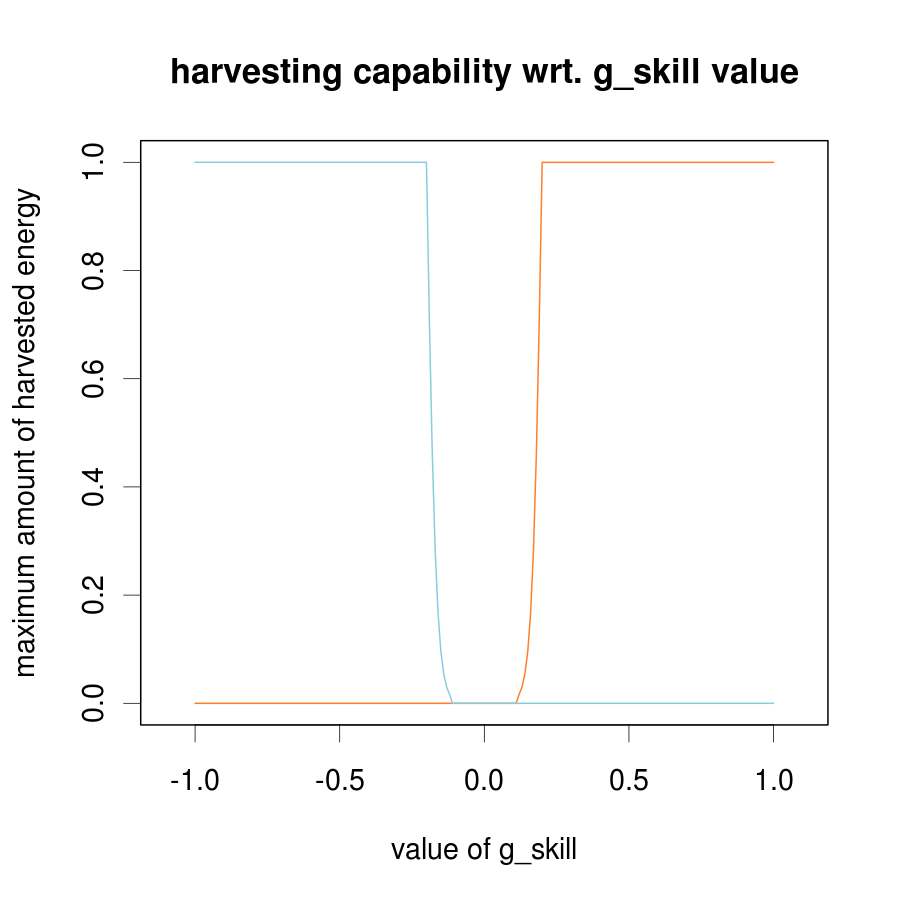
\includegraphics[width=.45\textwidth]{../images/sparsityEffect/f_skill}
\caption[Foraging Abilities]{Used function which said for each valu of $g_{skill}$ the amount of energy foraged. }

\label{fig:reward}

\end{figure}



\subsection{5 topologies}

Five different topologies based on :
\begin{description}
\item[Two resources dispositions ]:

\begin{description}
\item[Limited acces ]: La moitié des robots + 1 peut atteindre les deux resources, l'autre moitié +1 peut atteindre l'autre resource,  \label{it:1acc}
\item [Full access]: Les deux resources accessibles par tous les robots.\label{it:2acc}
\end{description}

\item[	Two robots dispositions]:
\begin{description}
\item[Chain]: Les robots sont en ligne et ne communiquent que deux à deux. \label{it:ligne}
\item[Two groups]: La population de robot est constituée de deux sous groupes qui ne peuvent communiquer entre eux que par le biais de deux robots. Au sein des sous groupes tous les robots peuvent communiquer.
.\label{it:2gp}
\end{description}
\end{description}

Which made five environnement:
\begin{table}[h]
\begin{tabular}{l|c|c|}
&robot disposition& resources disposition: \\
\hline
ENV0 &every robot can communicate& Full access\\\hline
ENV1 &Chain & Full access\\\hline
ENV2 &Chain & Limited access \\\hline
ENV3&Two groups & Full access\\\hline
ENV4&Two groups & Limited access 
\end{tabular}

\end{table}
\newcommand{\imgSize}{0.45\textwidth}
\begin{table}[h]
\caption{Five static environments}
\centering
\begin{tabular}{lcc}
&Full access&Limited acces\\
% \newline
all linked&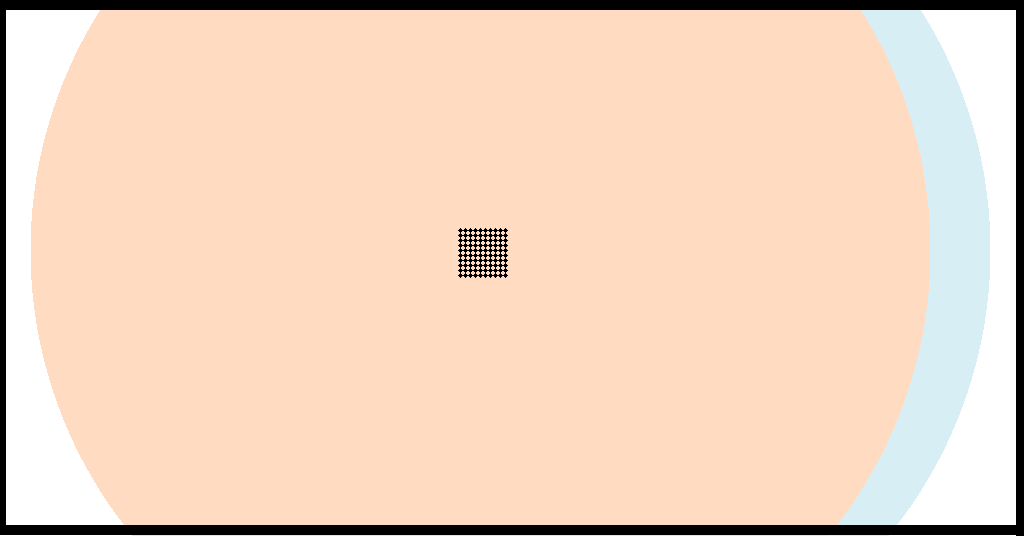
\includegraphics[width=\imgSize]{../images/5StaticEnv/environments/staticEnv0}&\\
% \newline
Two groups&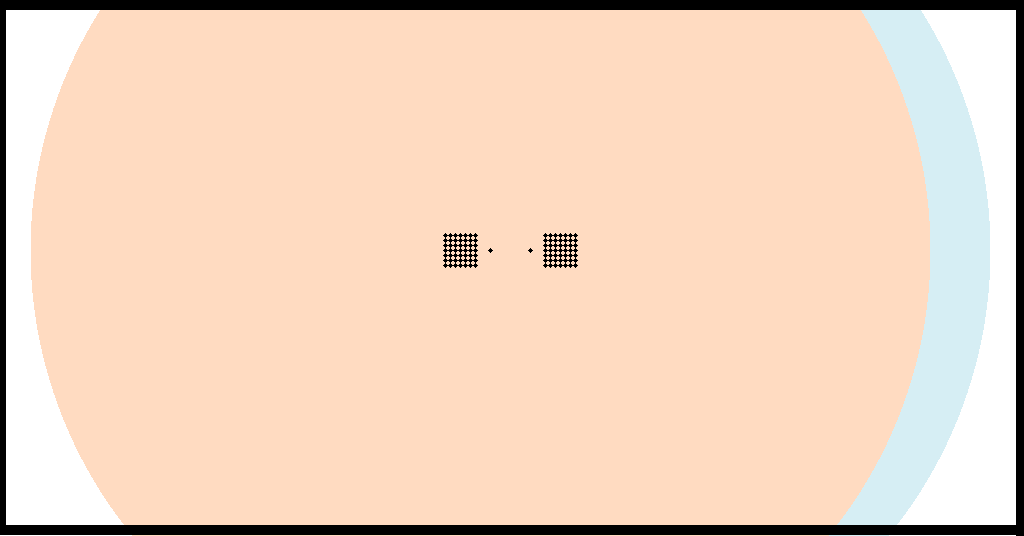
\includegraphics[width=\imgSize]{../images/5StaticEnv/environments/staticEnv3}&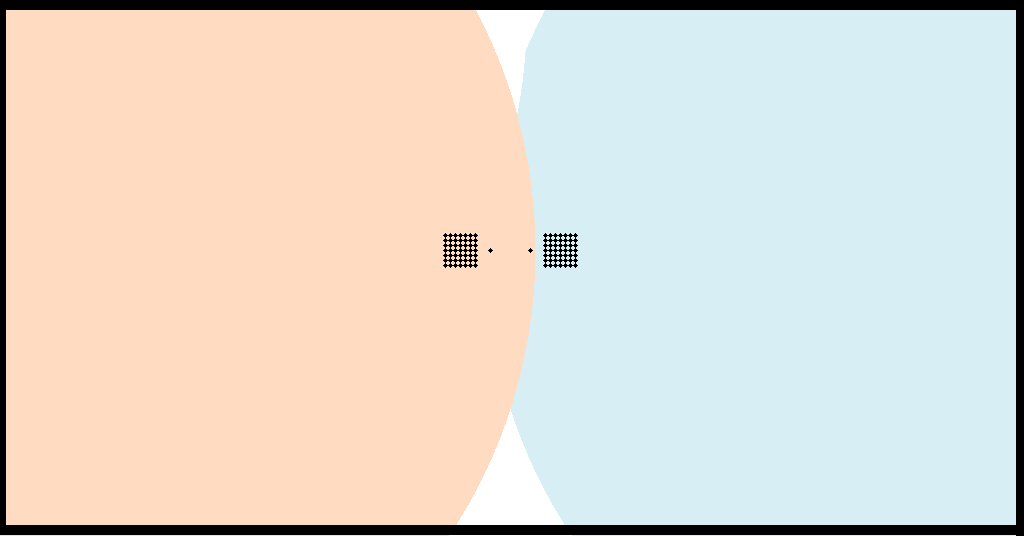
\includegraphics[width=\imgSize]{../images/5StaticEnv/environments/staticEnv4}\\
% \newline
Chain&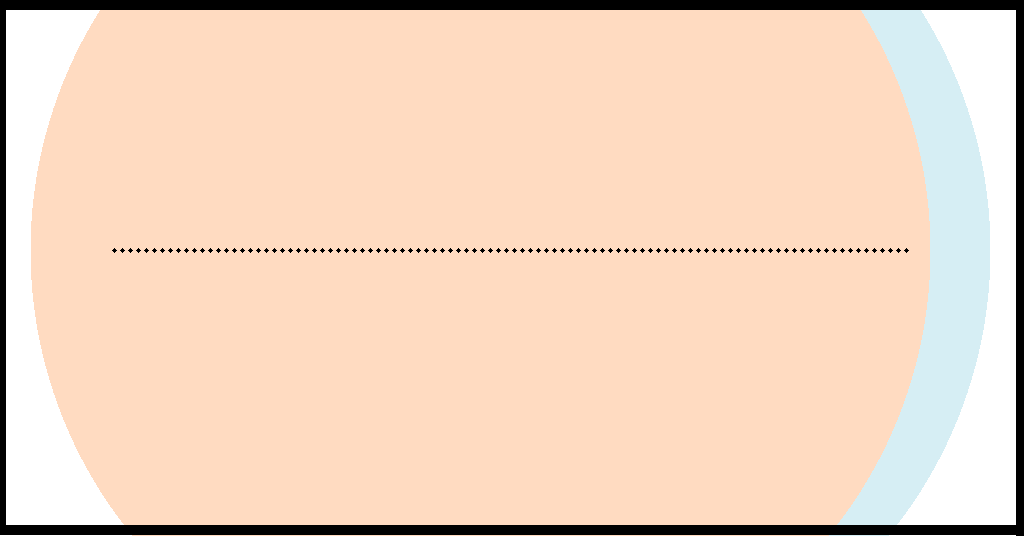
\includegraphics[width=\imgSize]{../images/5StaticEnv/environments/staticEnv1}&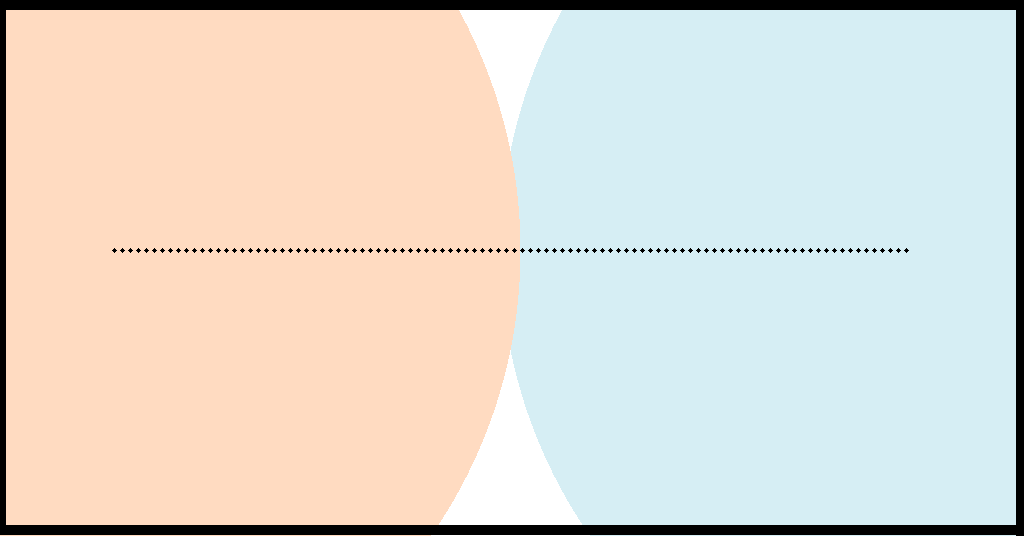
\includegraphics[width=\imgSize]{../images/5StaticEnv/environments/staticEnv2}\\
\end{tabular}
\label{tab:gt}

\end{table}%

\subsection{Exhaustive analyse of sparsity's effect}
The connexion between the agents are defined by a network builded as follow :
\begin{algorithm}
\caption{Network Generator}\label{alg:netGen}
\begin{algorithmic}

\WHILE {$currentSparsity\geq wSparsity$} 
\STATE $i\gets 0$
\IF {$currentSparsity+remainingEdgeToConnect() \leq wSparsity$}
\STATE $connectUnconnectedSubgraph()$
\ELSE
\STATE $randomlyconnectTwoNodes()$
\ENDIF
\STATE $updateSparsity()$
\ENDWHILE
\end{algorithmic}
\end{algorithm}

The networks generated by this algorithm are connexe. Some examples are given in figure \ref{fig:netEx}
\begin{figure}[H]
\caption{Example of networks generated by the generator (cf Algorithm \ref{alg:netGen}) for different sparsities}
\centering
\begin{tabular}{lc}
sparsity&One network for the given sparsity\\
% \newline
$0.01$&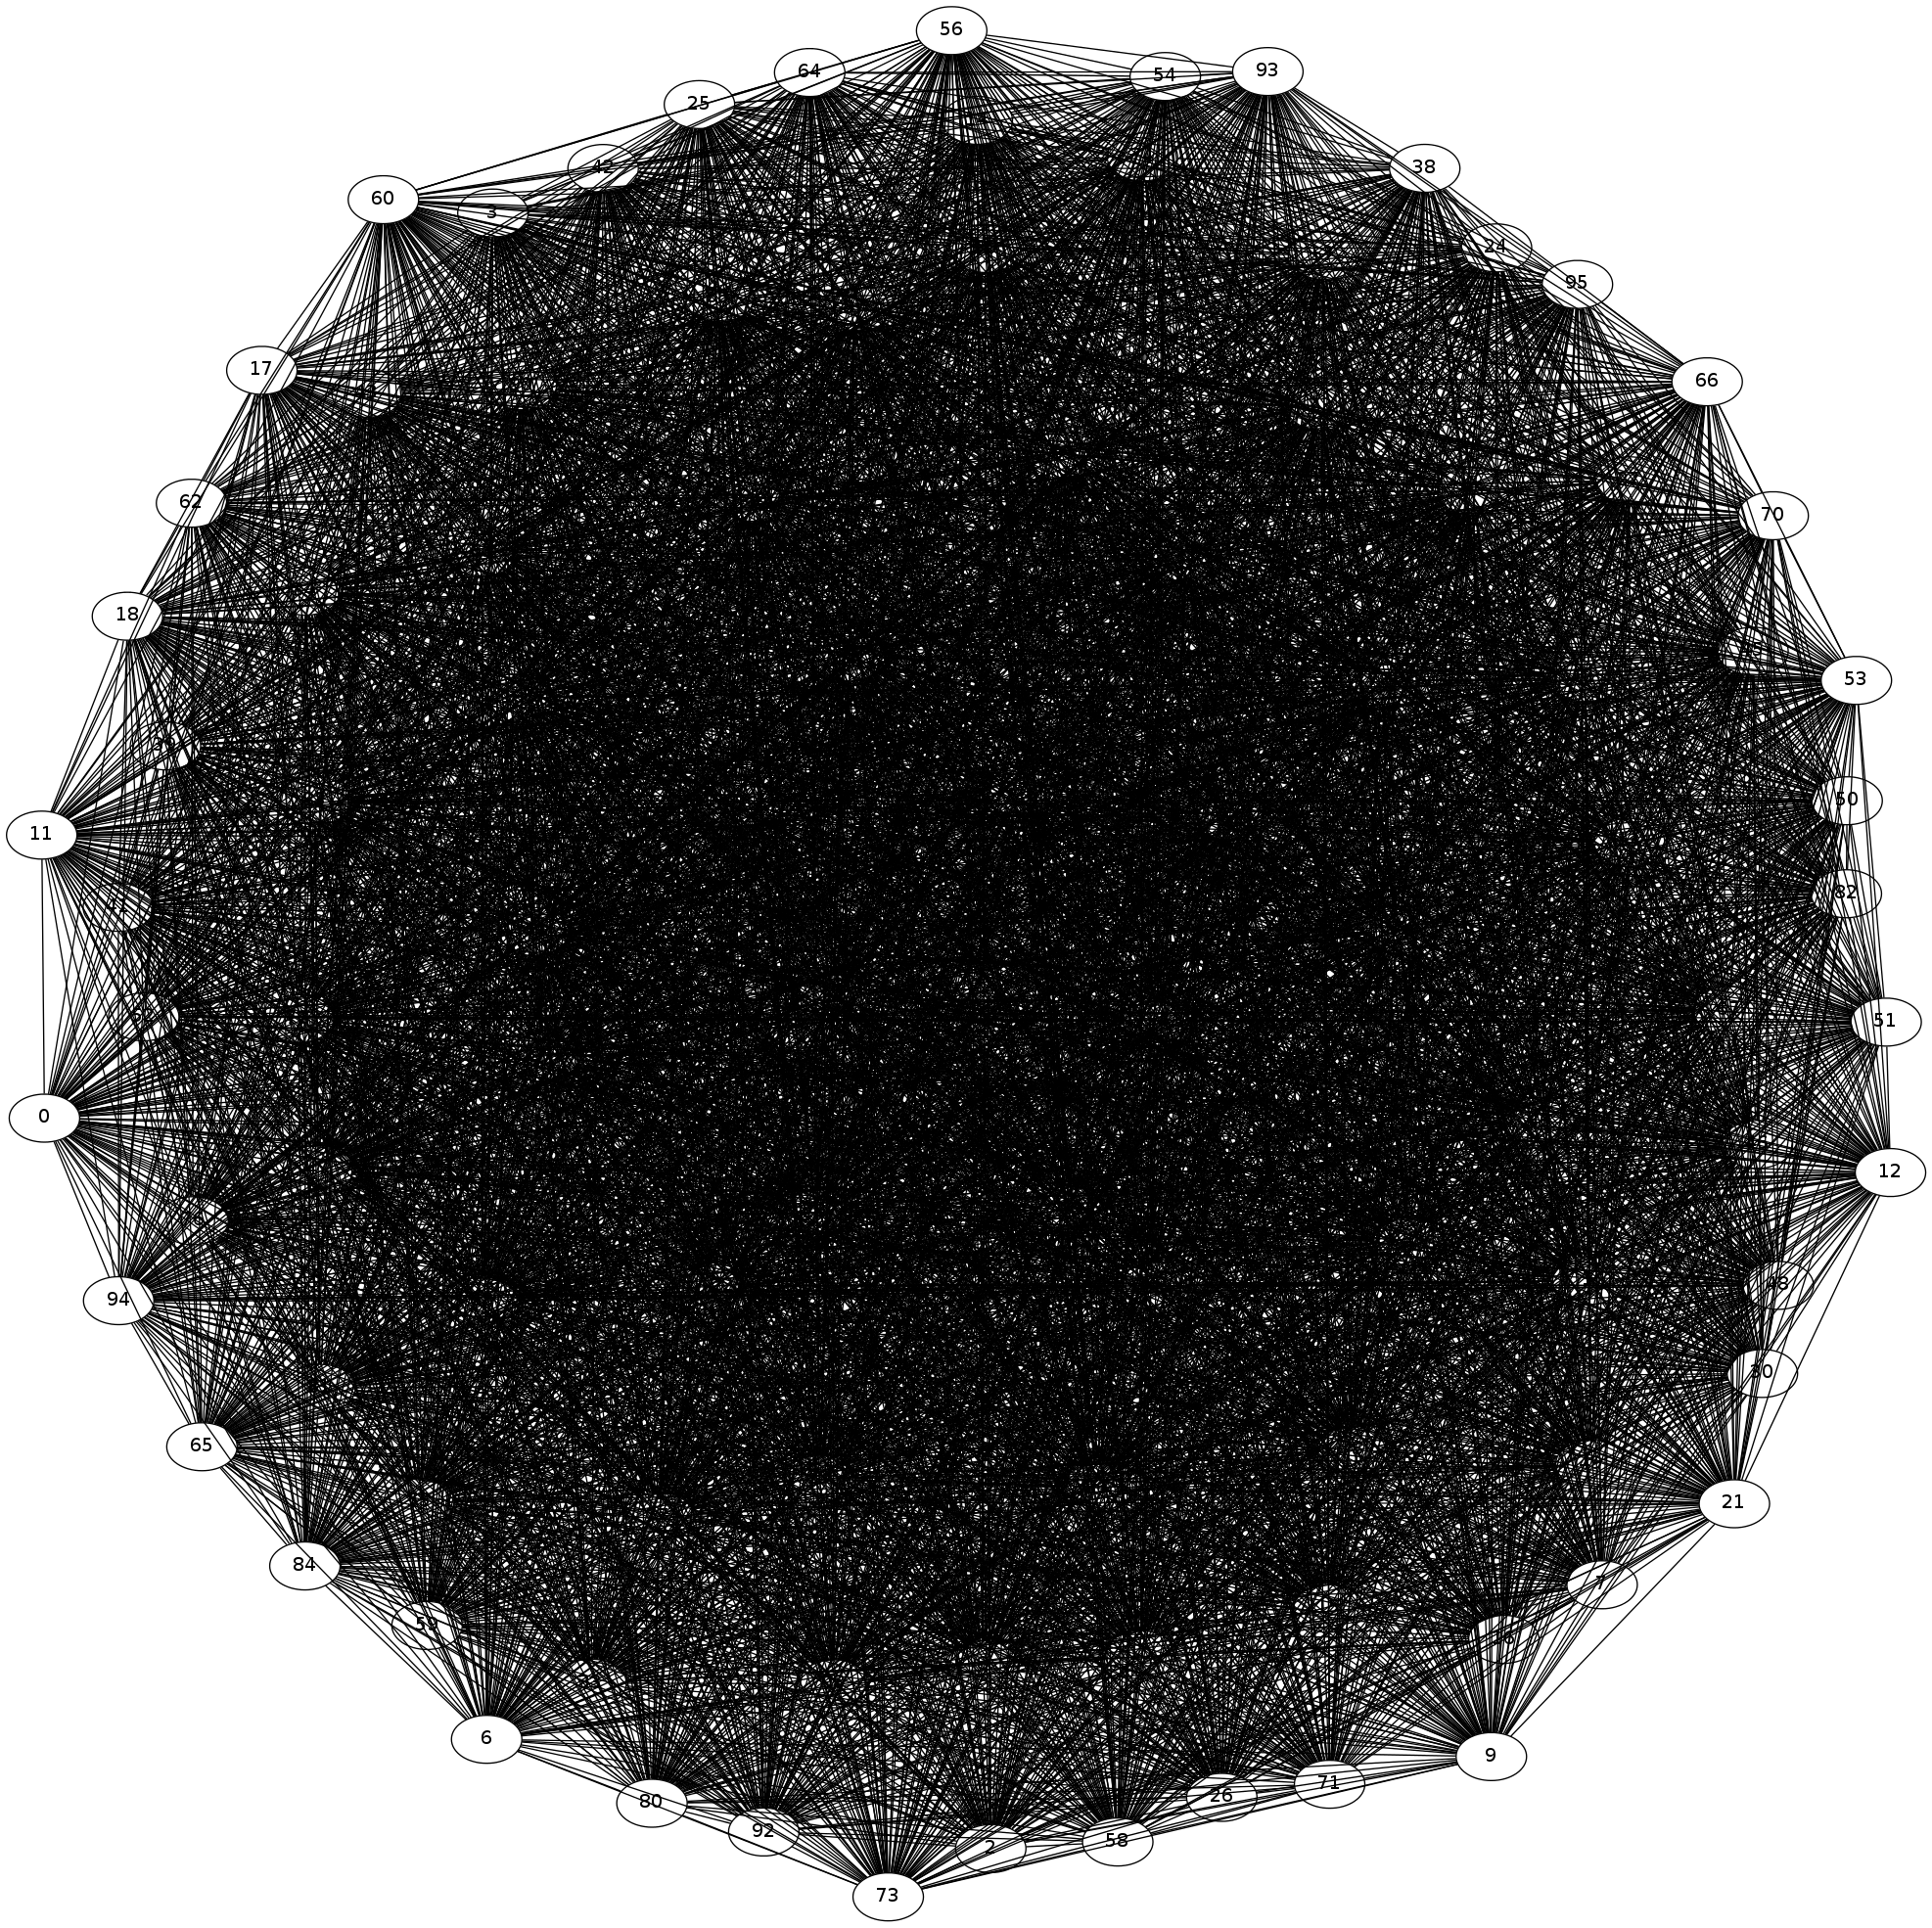
\includegraphics[width=\imgSize]{images/networks/neato_Network_sparsity1.png}\\
% \newline
$0.50$&\includegraphics[width=\imgSize]{images/networks/neato_Network_sparsity50.png}\\
% \newline
$0.98$&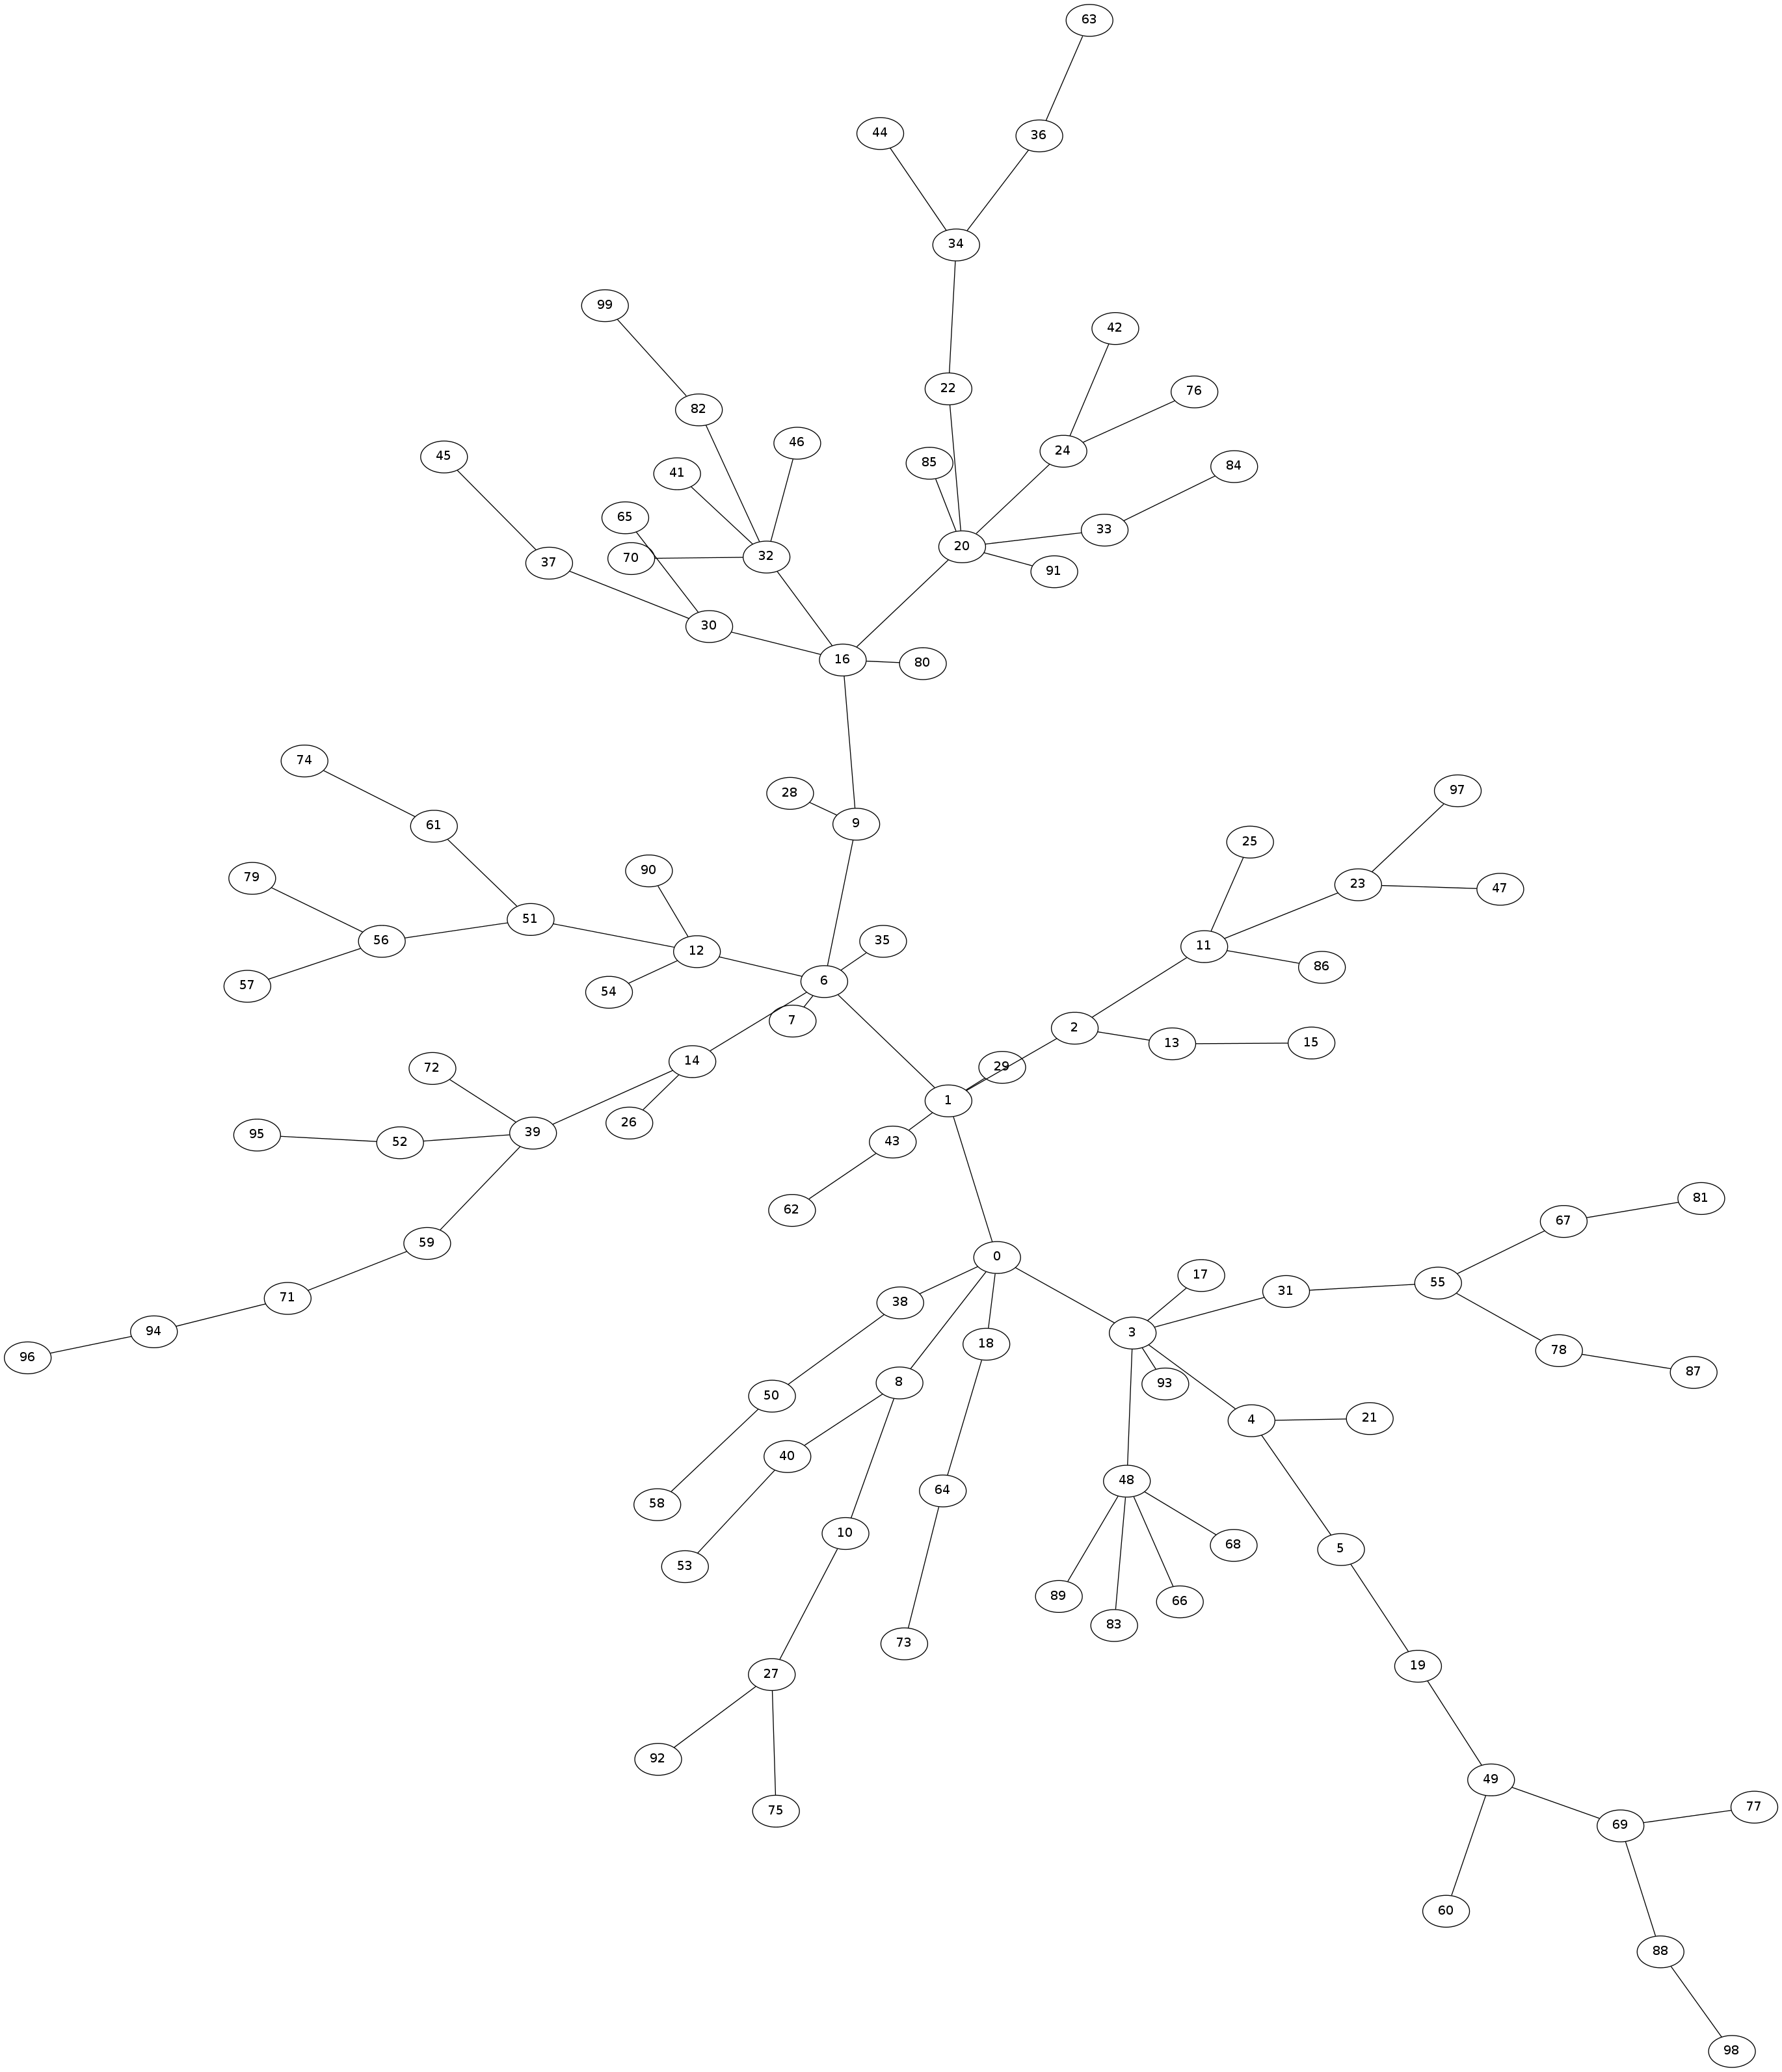
\includegraphics[width=\imgSize]{images/networks/neato_Network_sparsity98.png}\\
\end{tabular}
\label{fig:netEx}

\end{figure}%
\section{Results}

\subsection{In moving environnement}

\subsection{In five typical fixed topologies}


\subsubsection{Static environment 0}
% All robots are on the same place, can exchanges their genome and use both resources.
% Even here it works pretty well :

\begin{table}[H]
\caption{results for env0. \newline 
The top right graph show number of active robots during a 150\,000 iteration's run with resource availability at 50/50. As we can see if we wait a long time we will oscillate beetwen the two specialised populations. 
\newline The two middle graphs illustrate the same thing : the ratio beetwen the number of individu foraging R1 and the ration of individu which exploit R2 at the end of a run. And this for all different resource repartitions .
\newline The two bottom graphs show the mean number (left graph) and the median(right graph) of active agents using R1 (dark grey) and r2 (light grey) respectively.}
\centering
\begin{tabular}{cc}
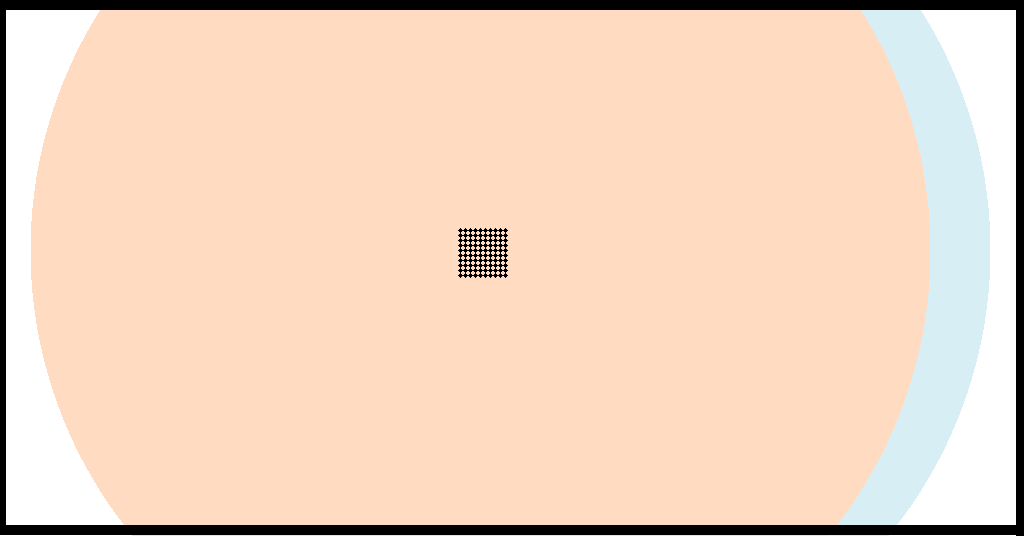
\includegraphics[width=\imgSize]{../images/5StaticEnv/environments/staticEnv0}&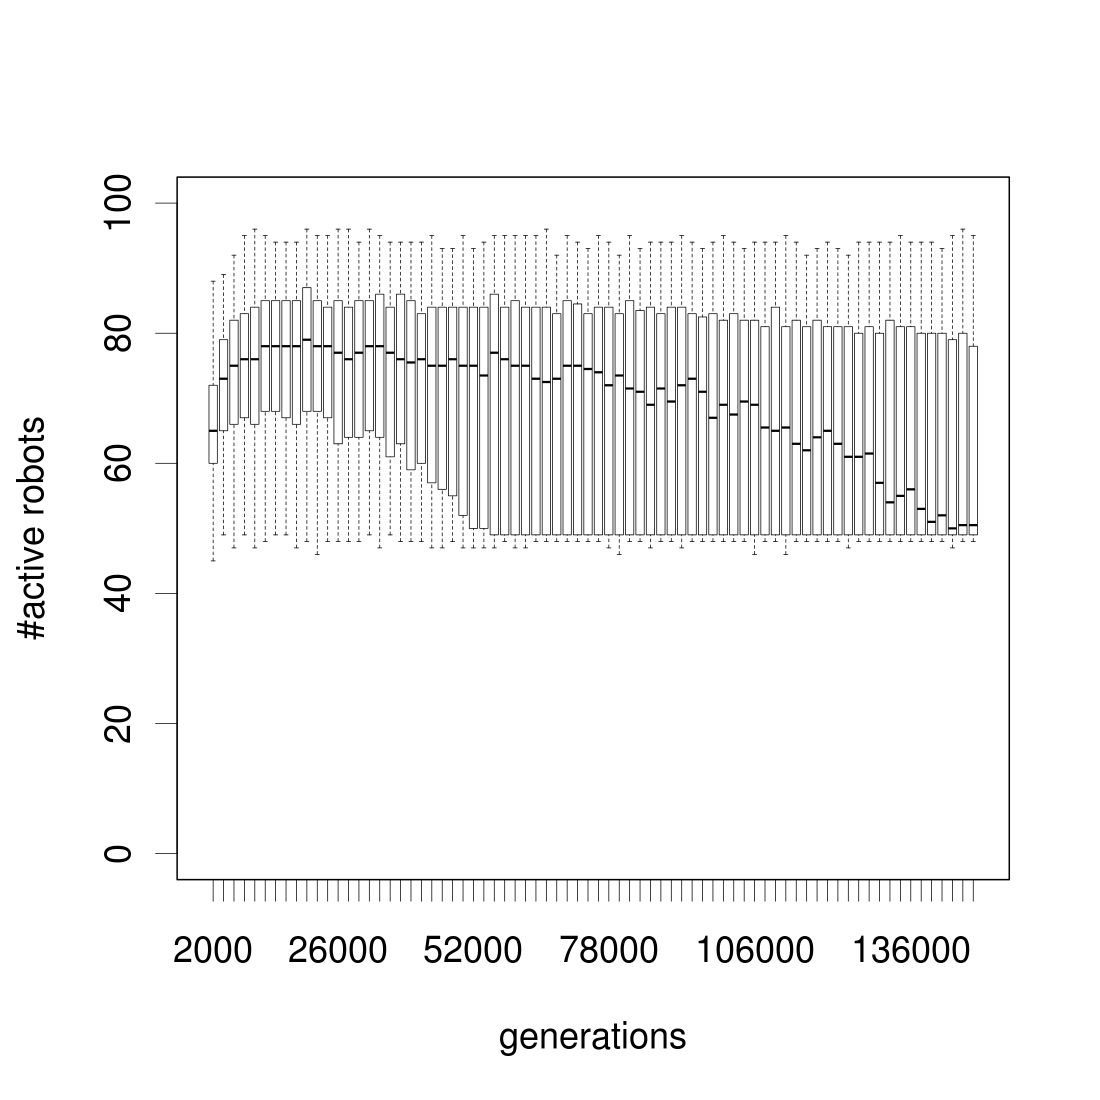
\includegraphics[width=\imgSize]{../images/5StaticEnv/alive_staticEnv0}\\
\newline
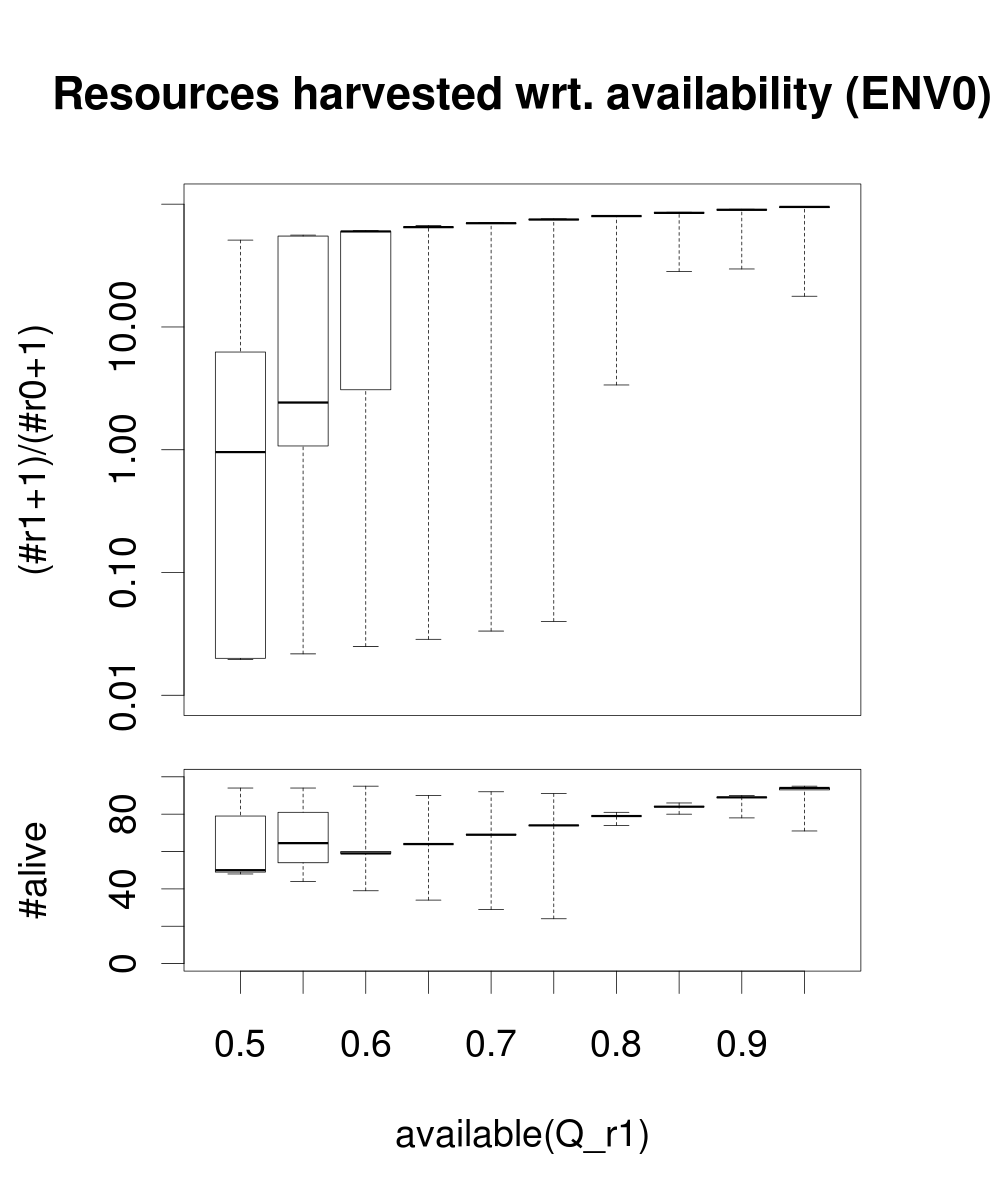
\includegraphics[width=\imgSize]{../images/5StaticEnv/ratioAndRep_staticEnv0LogY}& 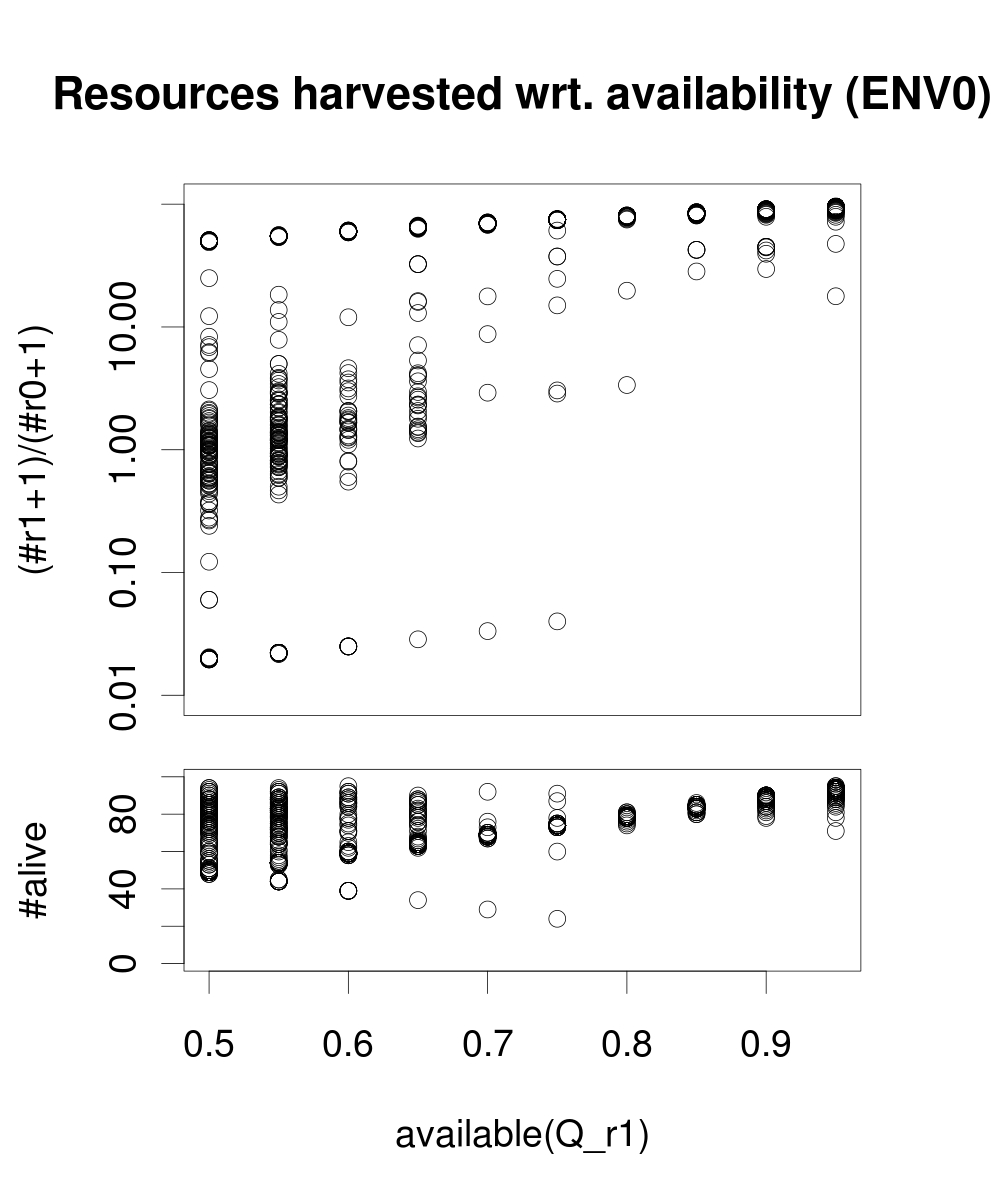
\includegraphics[width=\imgSize]{../images/5StaticEnv/ratioAndRep_staticEnvPlot0LogY}\\
\end{tabular}
\end{table}
\begin{table}[H]
\caption{Left graphs use mean values ; rights use the median.Bottom graphes are normalized}
\begin{tabular}{cc}
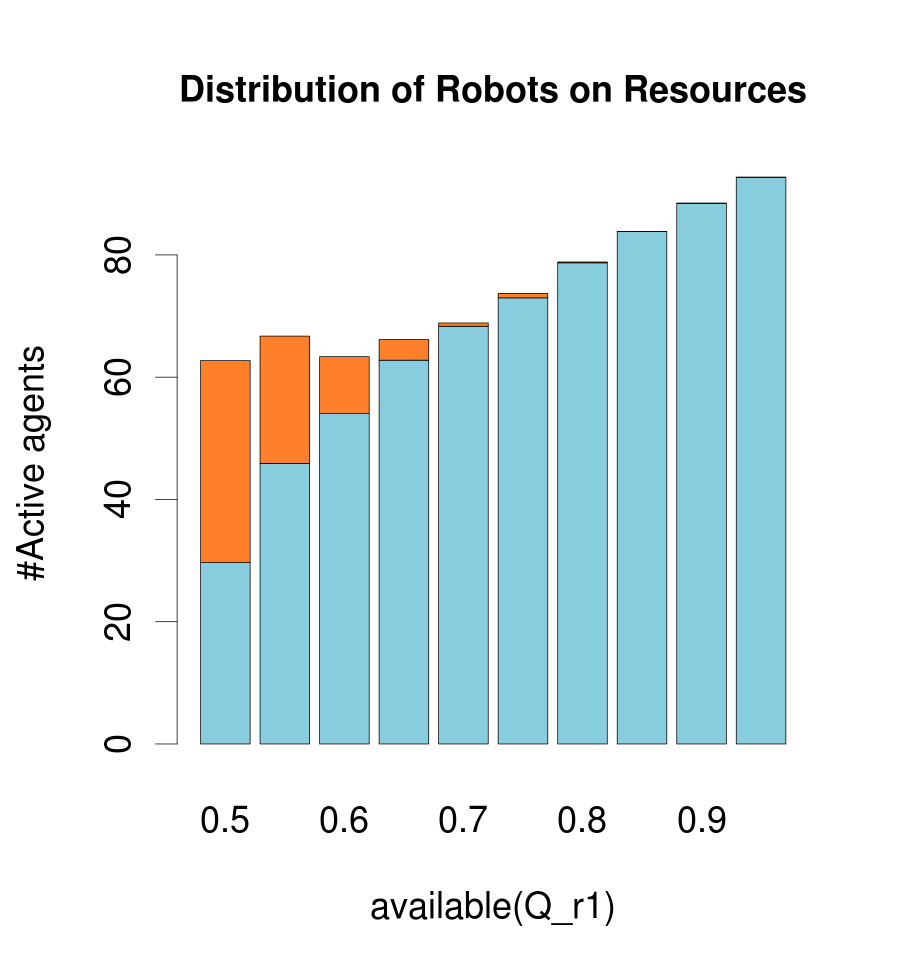
\includegraphics[width=\imgSize]{../images/5StaticEnv/barplotAliveR1AndR2_mean_env0}& 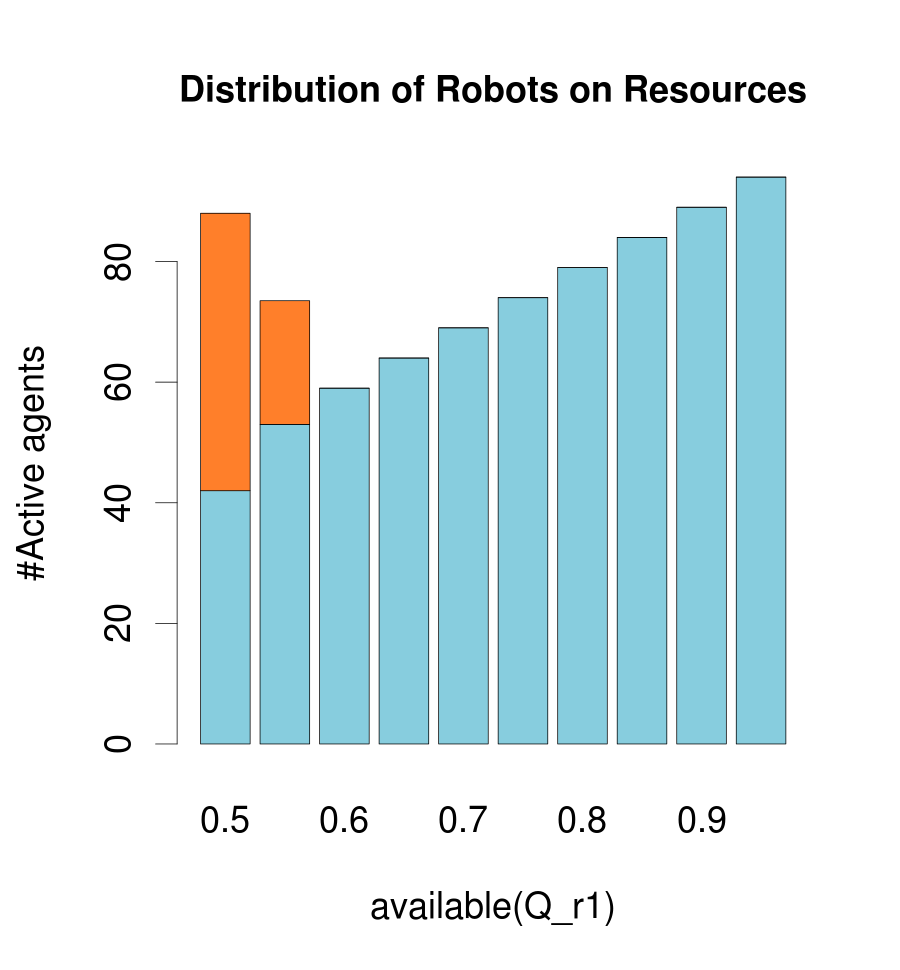
\includegraphics[width=\imgSize]{../images/5StaticEnv/barplotAliveR1AndR2_median_env0}\\
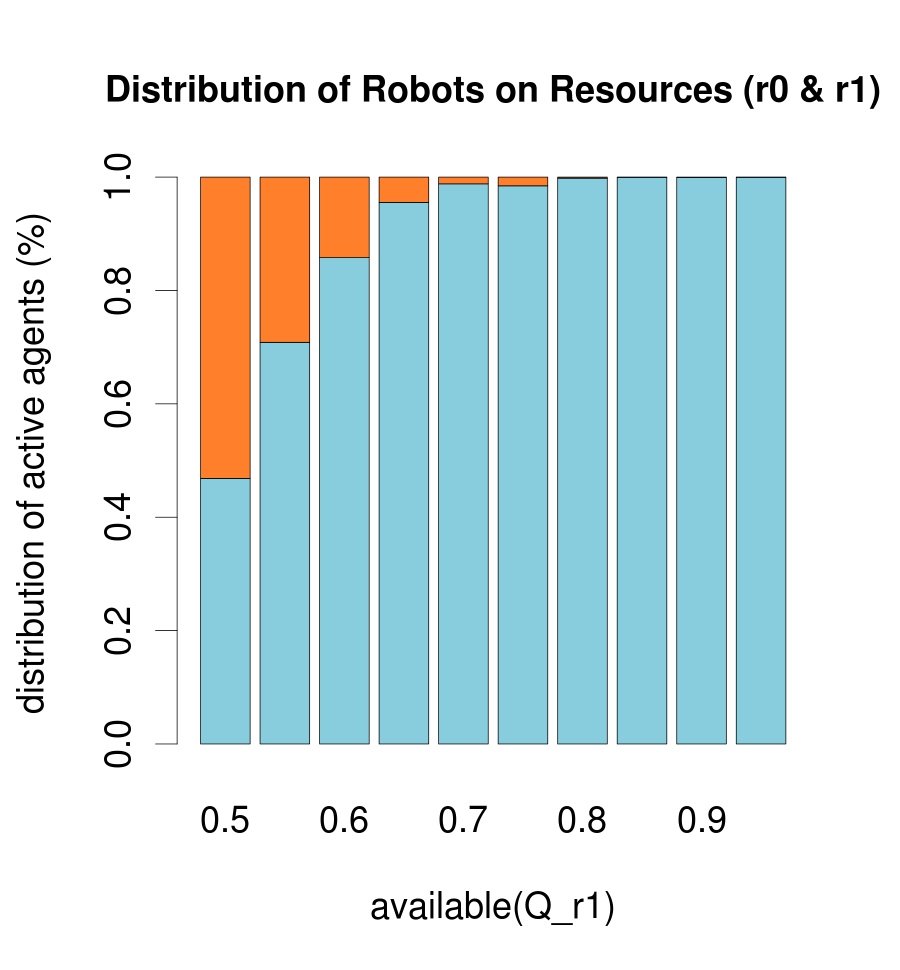
\includegraphics[width=\imgSize]{../images/5StaticEnv/barplotAliveR1AndR2_mean_env0_normalized}& 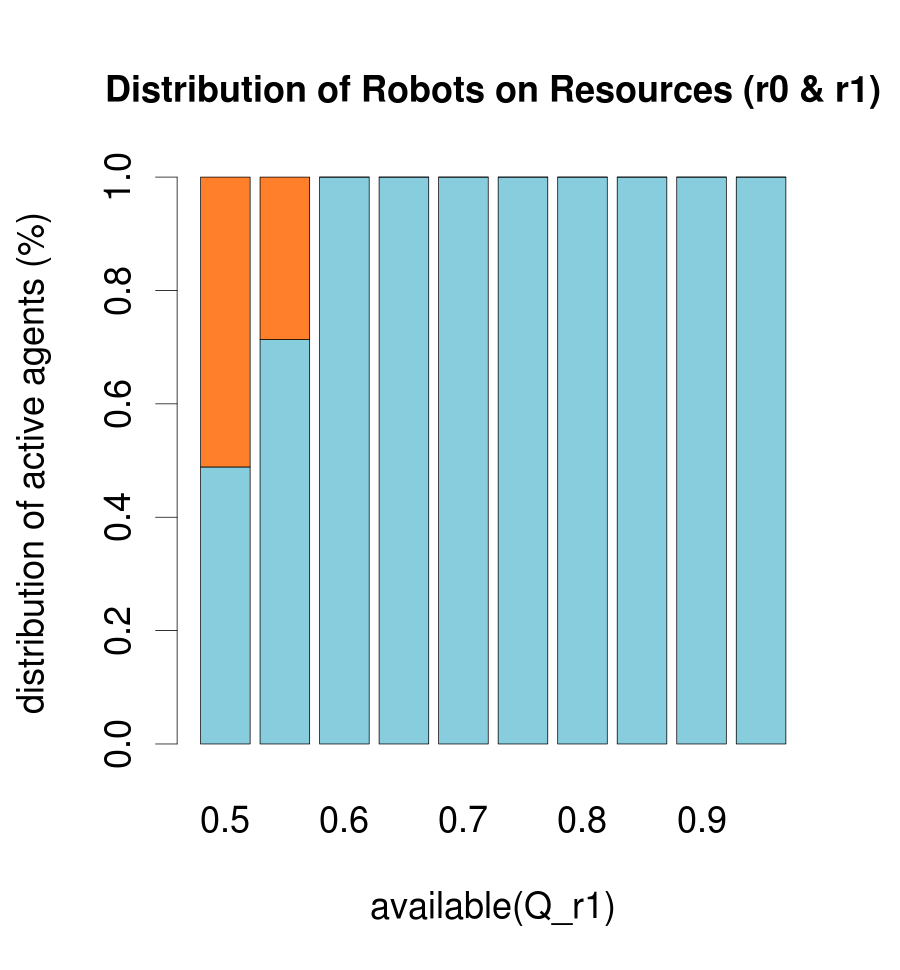
\includegraphics[width=\imgSize]{../images/5StaticEnv/barplotAliveR1AndR2_median_env0_normalized}\\
\end{tabular}
\end{table}
% \vspace{-1cm}
\begin{table}[H]
\caption{Environment 0, Samples:\\On the left : the repartition of $g_{skill}$ in the whole population during the time ; on the right : the value of $g_{skill}$ for all robot during the time. }
\centering
\begin{tabular}{cc}
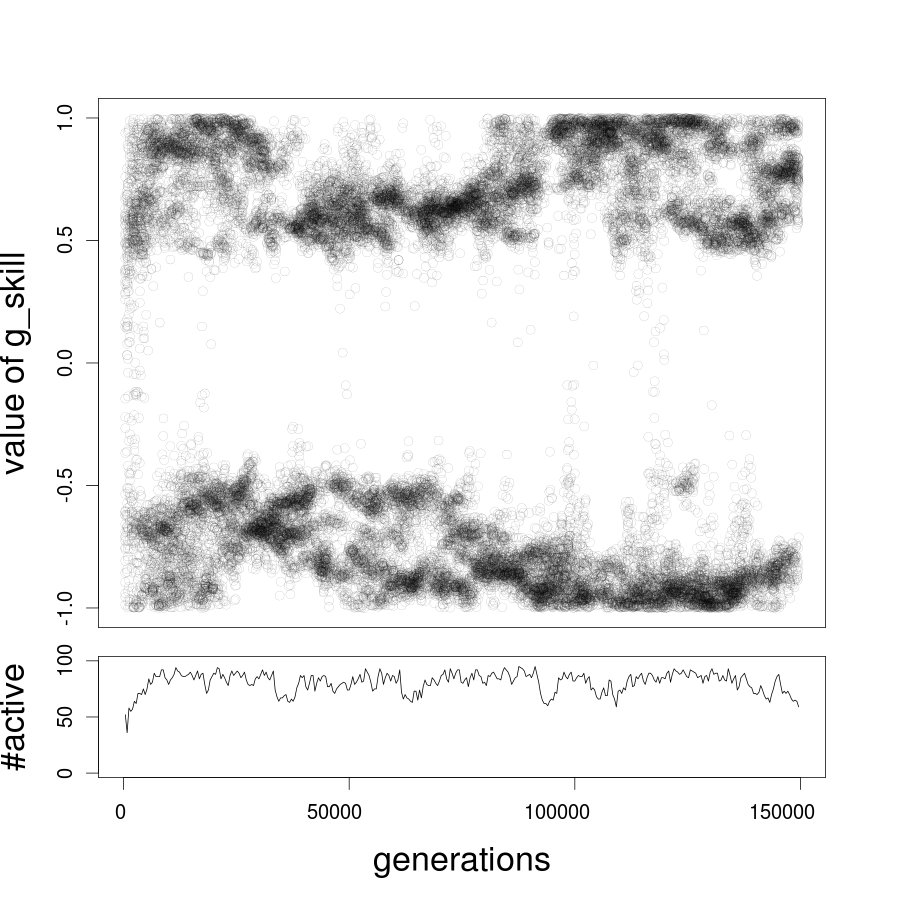
\includegraphics[width=\imgSize]{../images/5StaticEnv/Gplot59_staticEnv0}&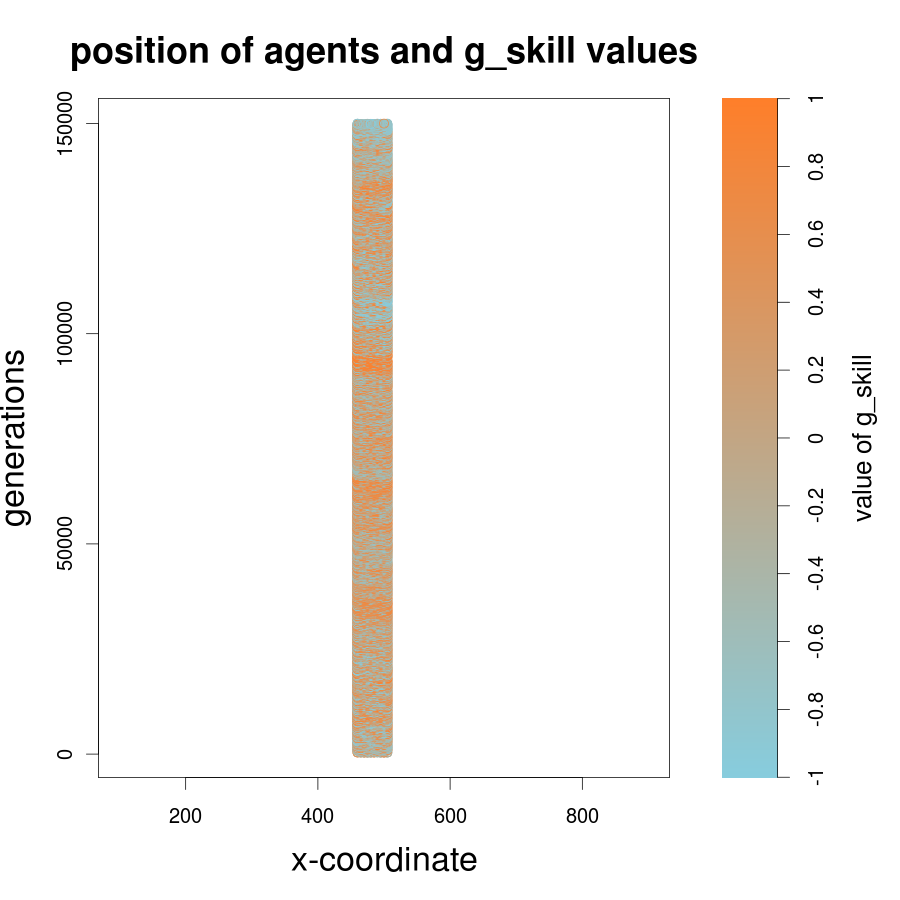
\includegraphics[width=\imgSize]{../images/5StaticEnv/Gplot59Static_staticEnv0}\\
\newline
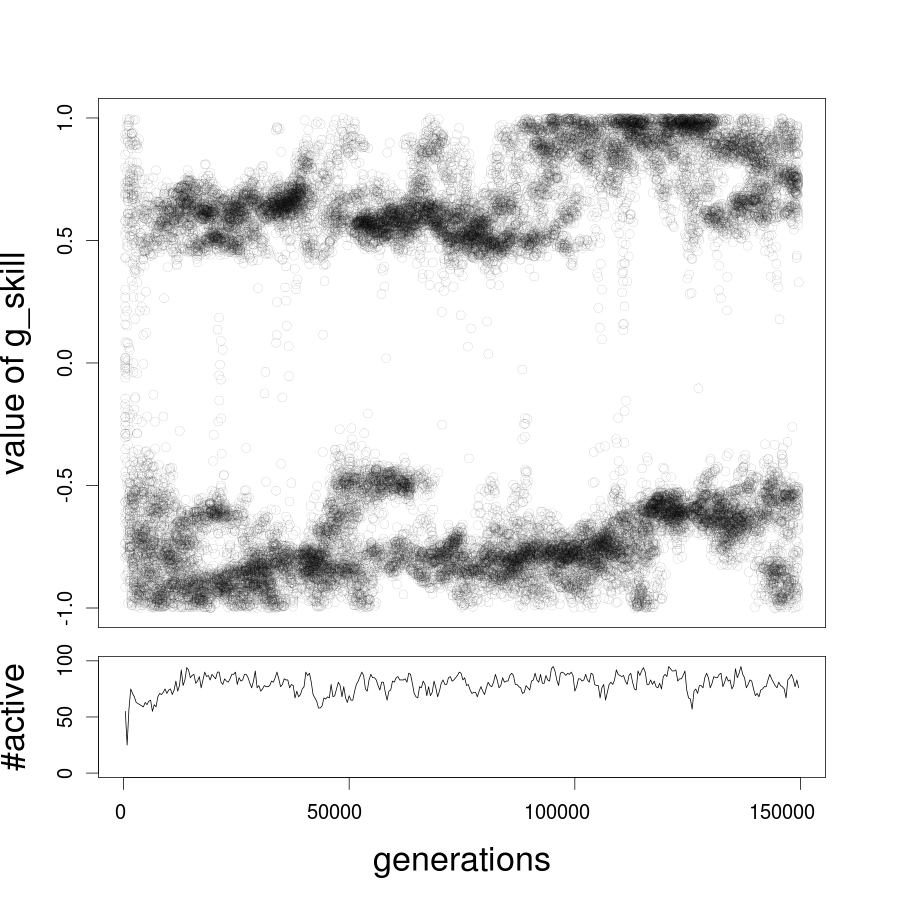
\includegraphics[width=\imgSize]{../images/5StaticEnv/Gplot47_staticEnv0}&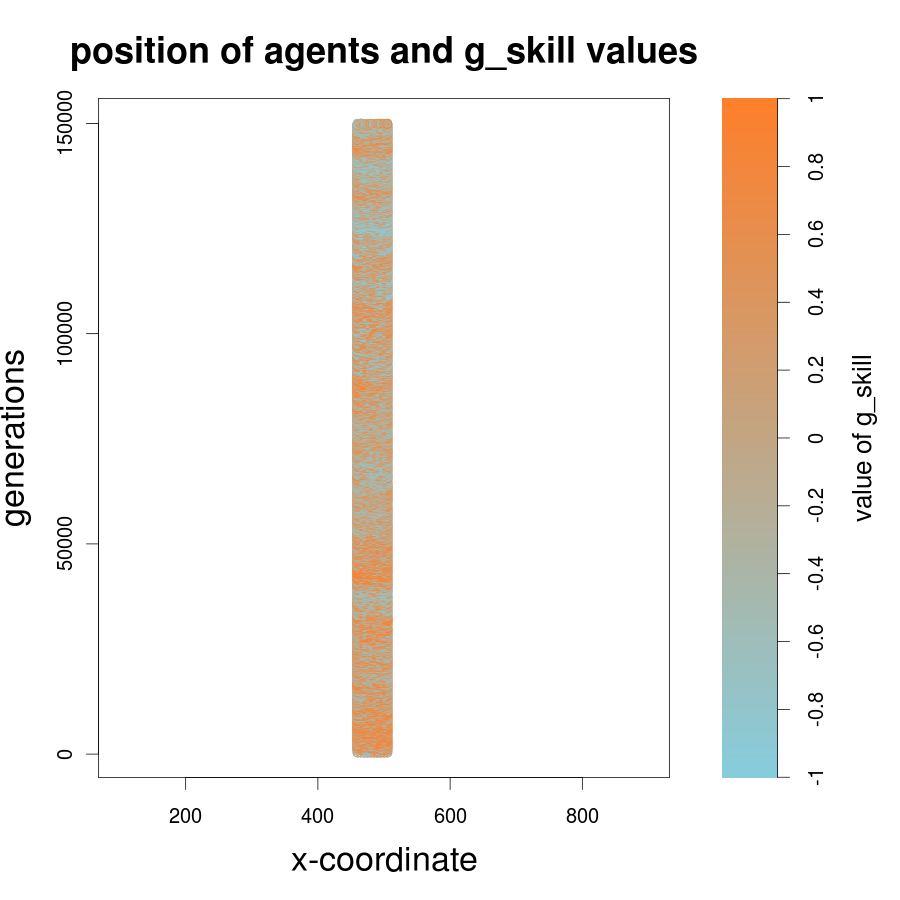
\includegraphics[width=\imgSize]{../images/5StaticEnv/Gplot47Static_staticEnv0}\\
\end{tabular}
\end{table}
\begin{table}[H]
\begin{tabular}{cc}
 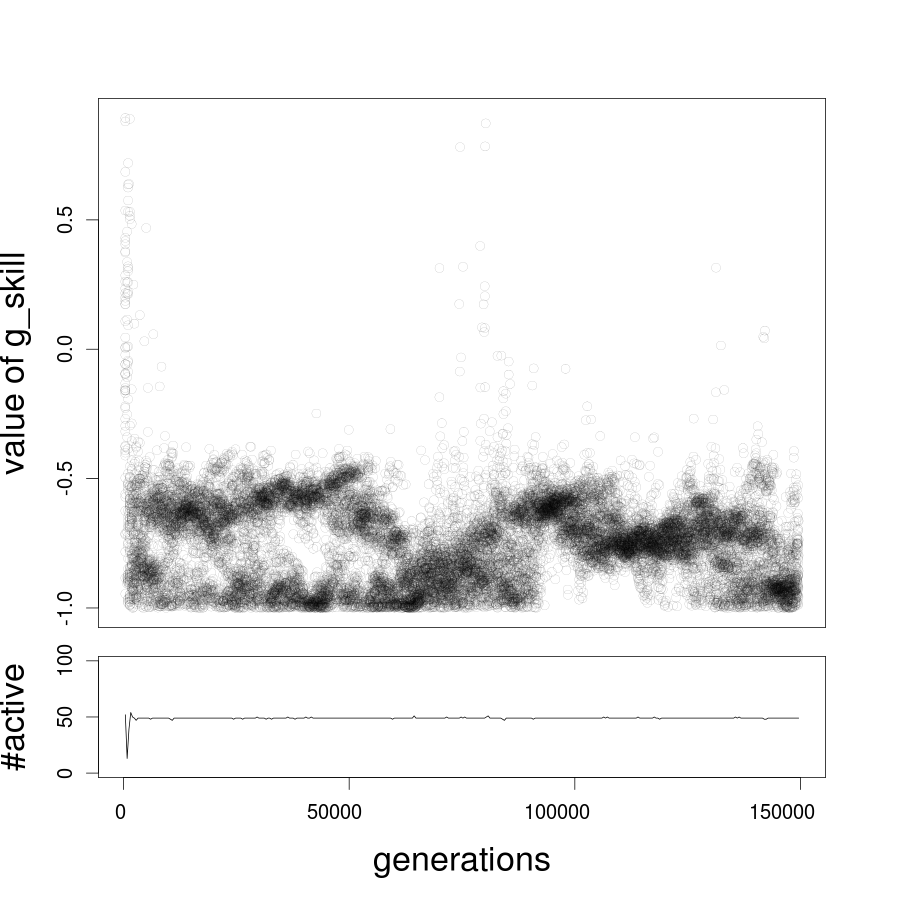
\includegraphics[width=\imgSize]{../images/5StaticEnv/Gplot62_staticEnv0}&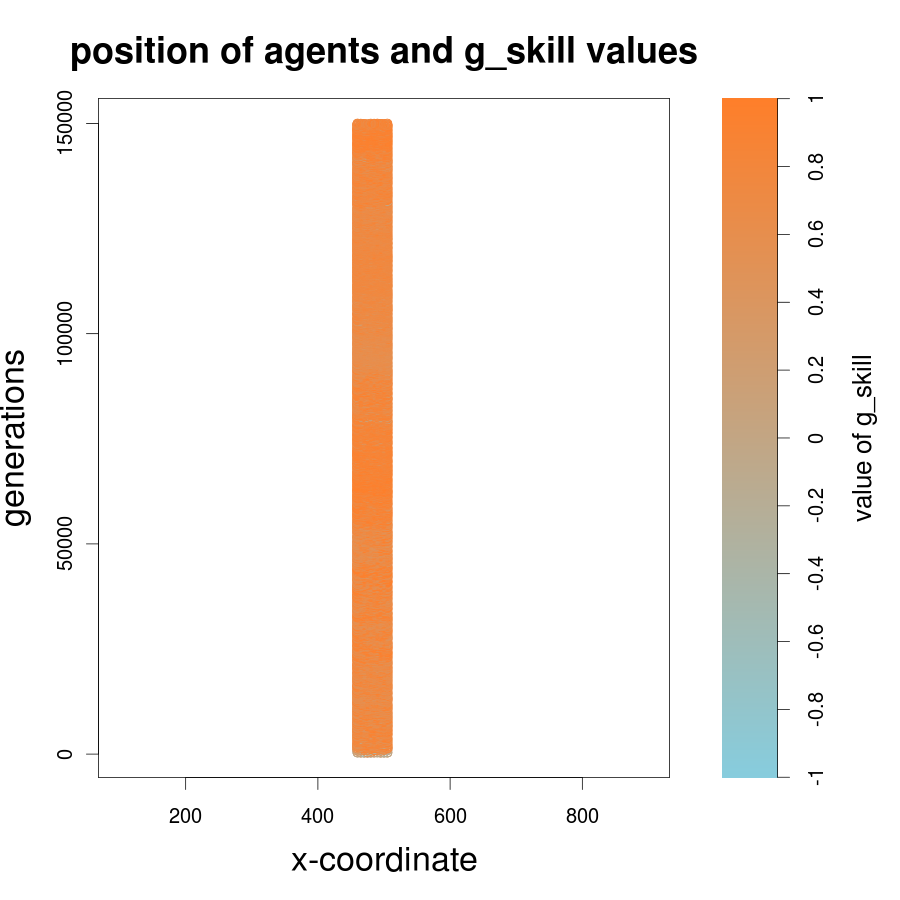
\includegraphics[width=\imgSize]{../images/5StaticEnv/Gplot62Static_staticEnv0}\\
 \newline
 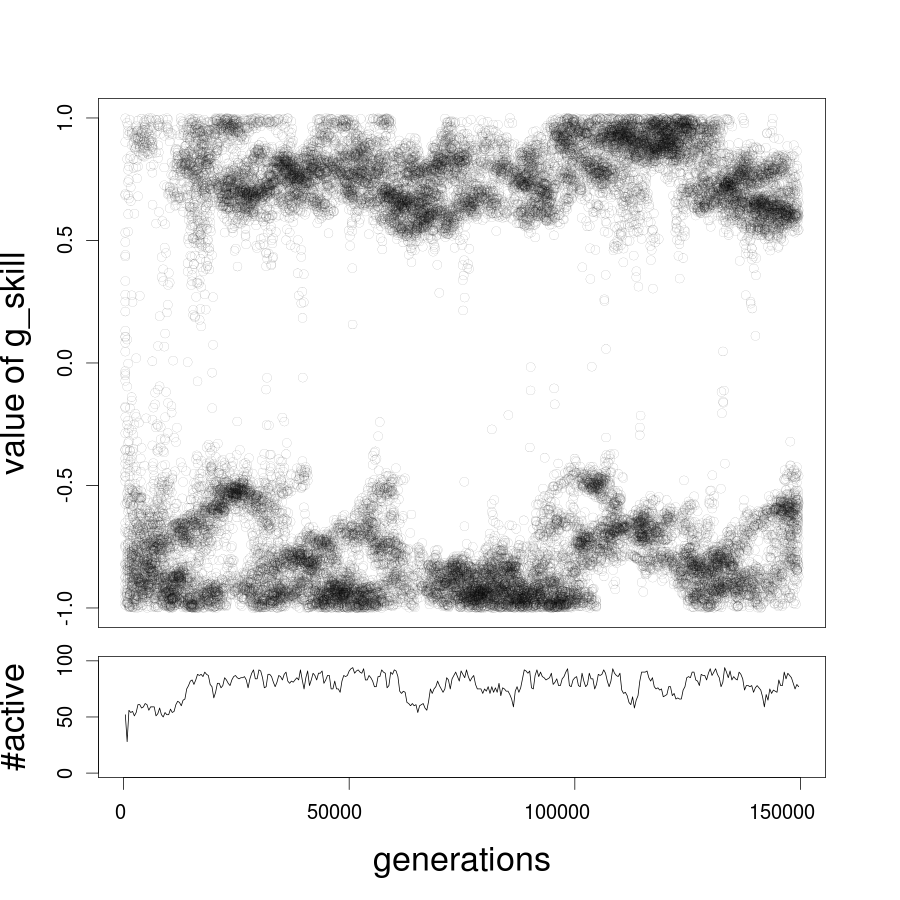
\includegraphics[width=\imgSize]{../images/5StaticEnv/Gplot58_staticEnv0}&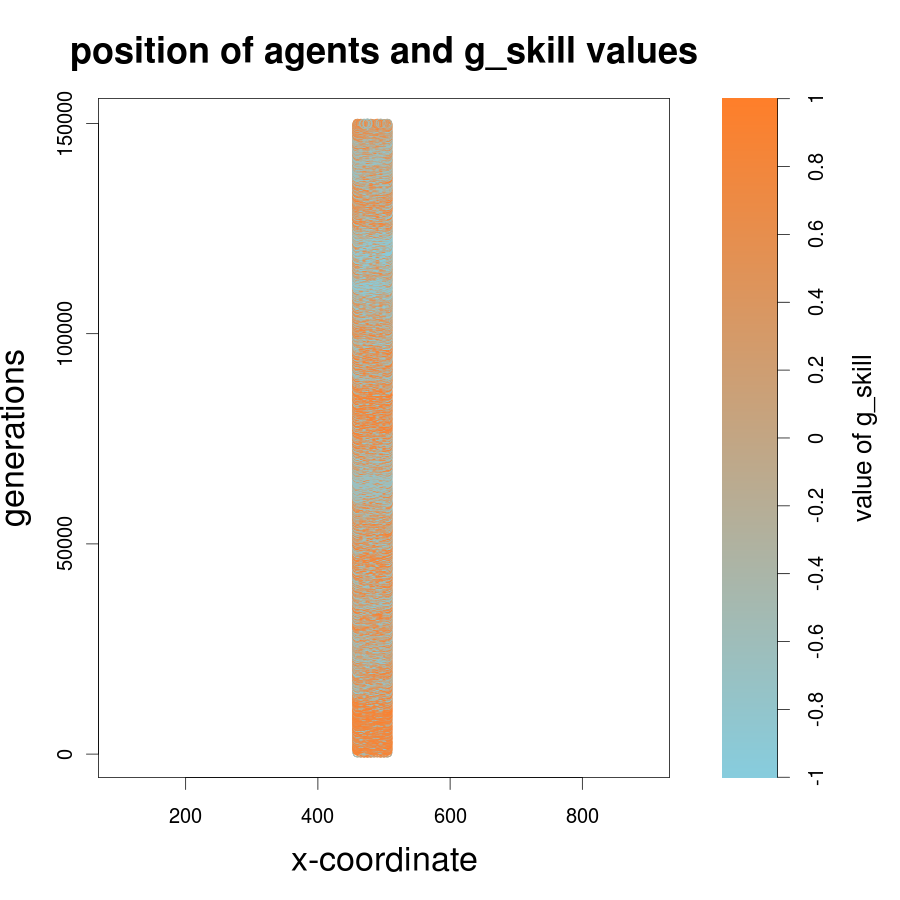
\includegraphics[width=\imgSize]{../images/5StaticEnv/Gplot58Static_staticEnv0}\\
\end{tabular}

\end{table}

\subsubsection{Static environment 1}
\begin{table}[H]
\caption{results for ENV1.\newline On the bottom left graph we see that it is more diffult to maintain the theoritical ratio when the smallest subpopulation cannot be larger than 20 percent of the population. After that the biggest population overcome the environment. }
\centering
\begin{tabular}{cc}
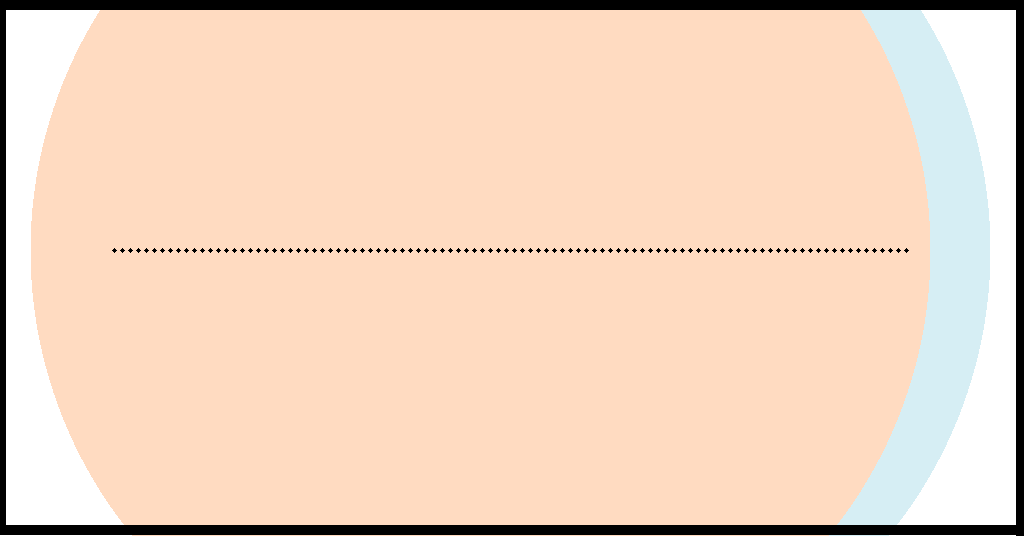
\includegraphics[width=\imgSize]{../images/5StaticEnv/environments/staticEnv1}&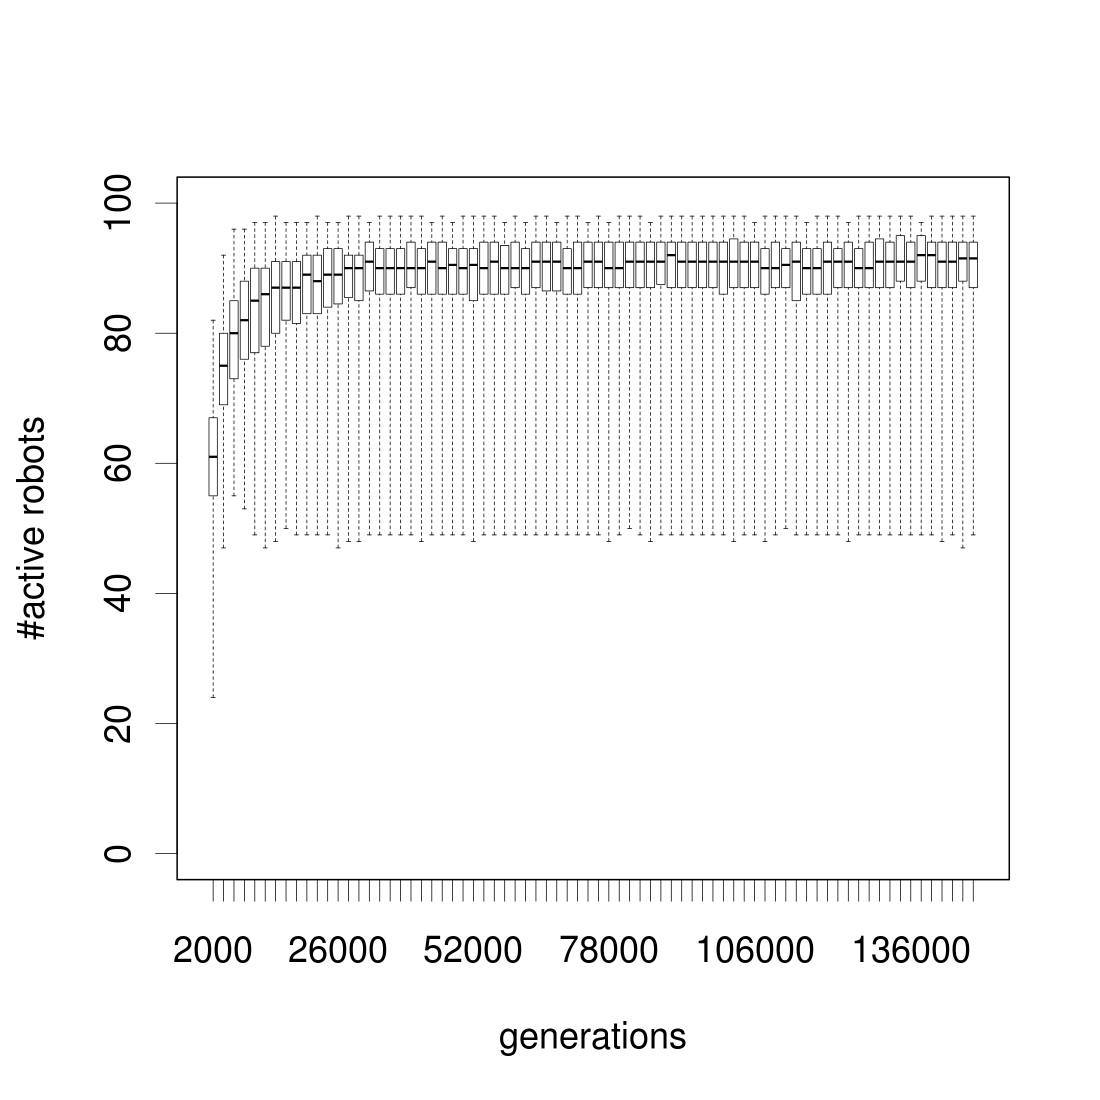
\includegraphics[width=\imgSize]{../images/5StaticEnv/alive_staticEnv1}\\
\newline
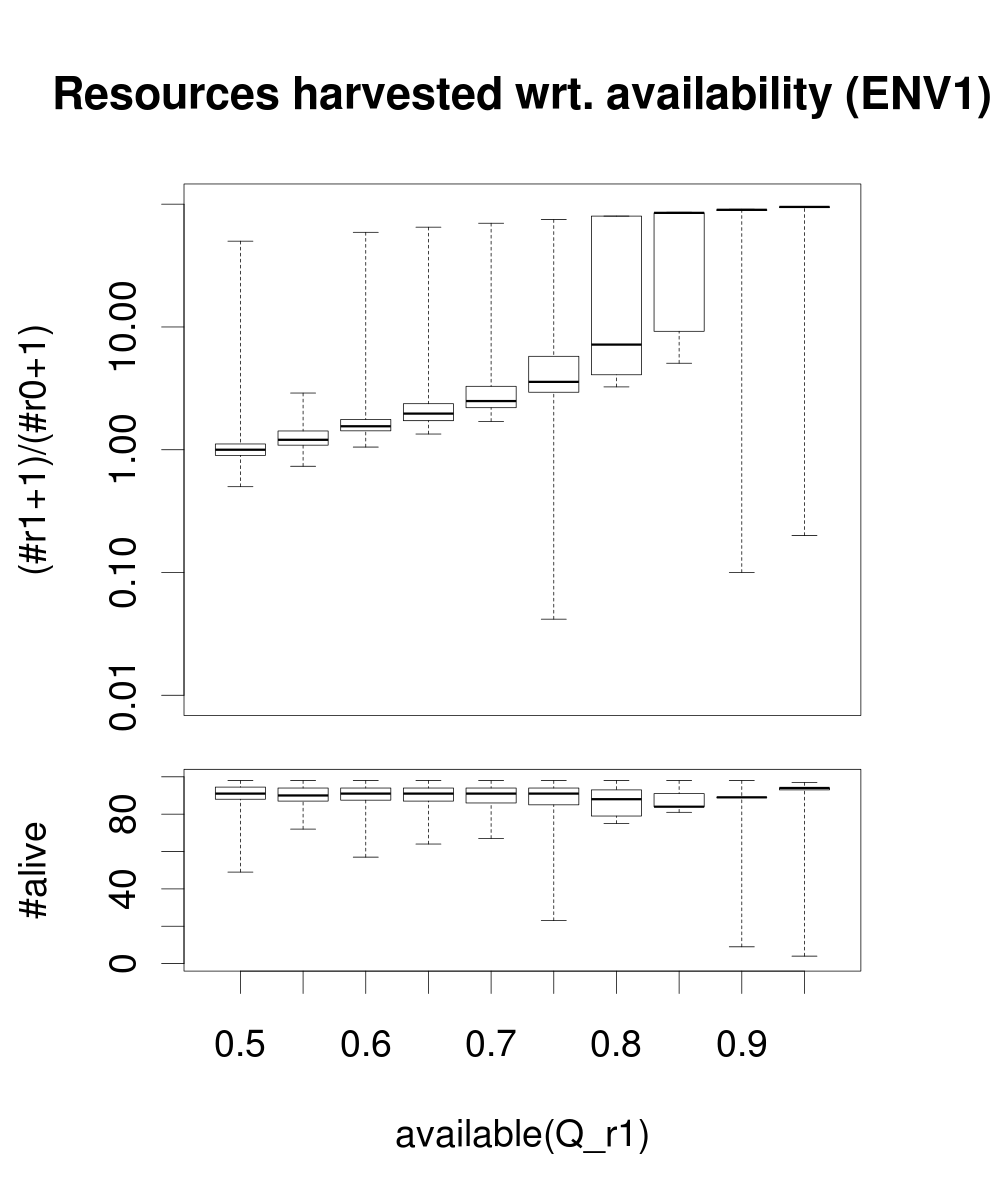
\includegraphics[width=\imgSize]{../images/5StaticEnv/ratioAndRep_staticEnv1LogY}&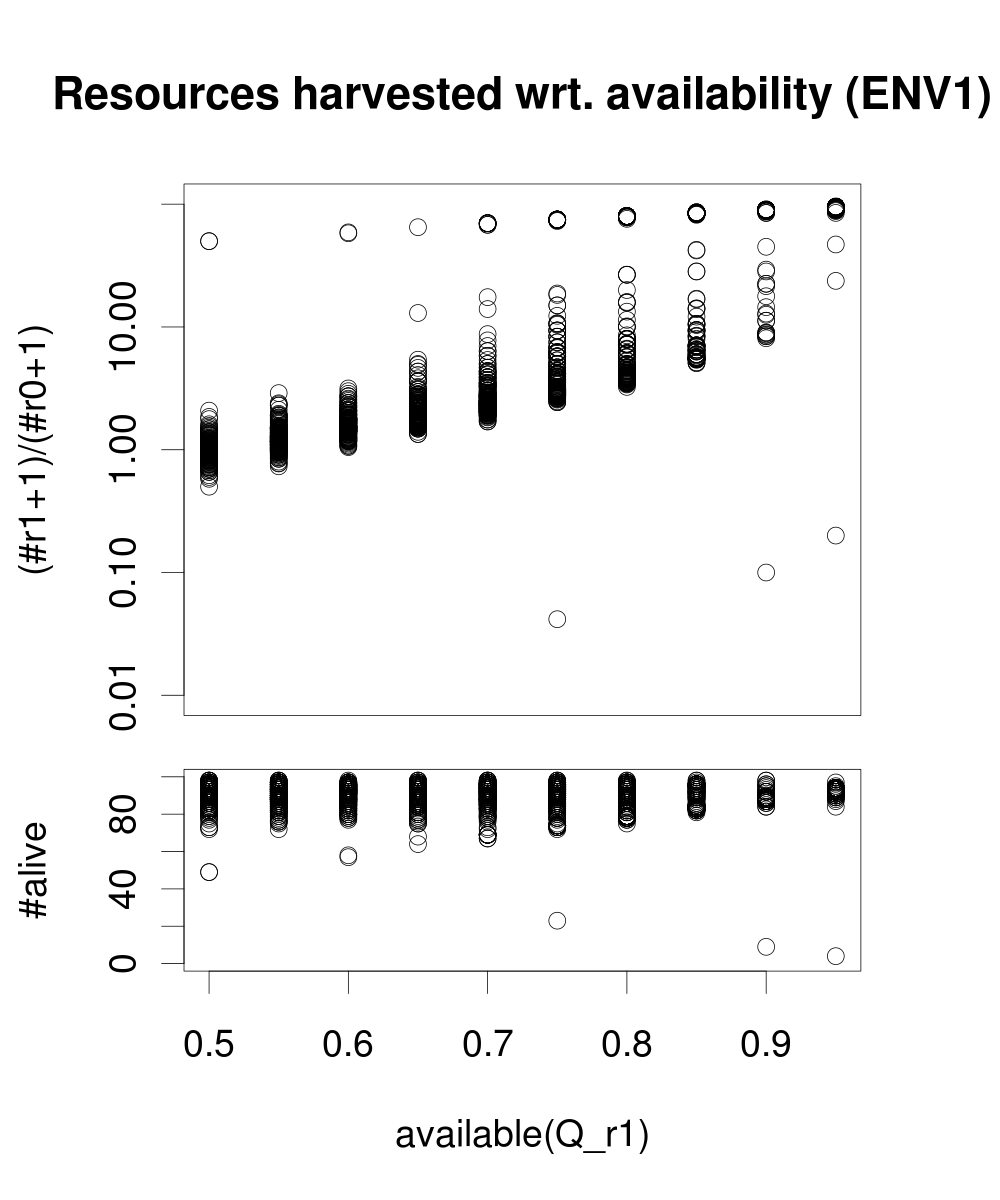
\includegraphics[width=\imgSize]{../images/5StaticEnv/ratioAndRep_staticEnvPlot1LogY}\\
\end{tabular}
\end{table}
\begin{table}[H]
\caption{Left graphs use mean values ; rights use the median.Bottom graphes are normalized}
\begin{tabular}{cc}

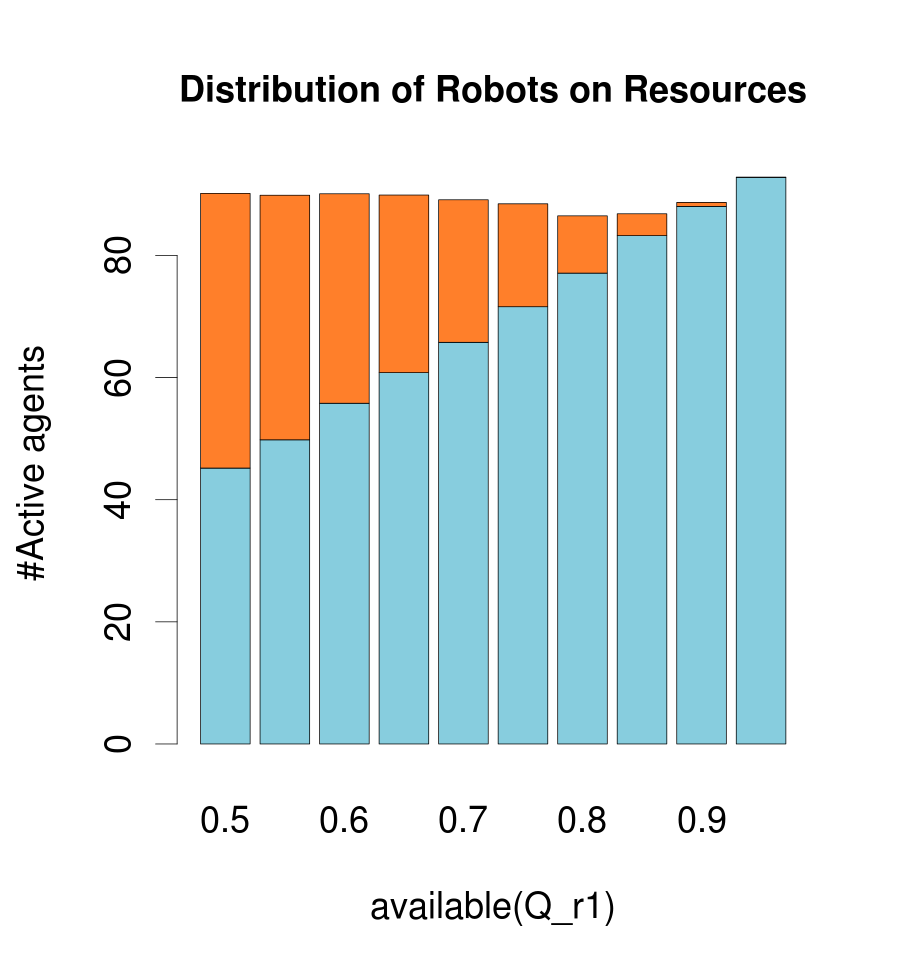
\includegraphics[width=\imgSize]{../images/5StaticEnv/barplotAliveR1AndR2_mean_env1}& 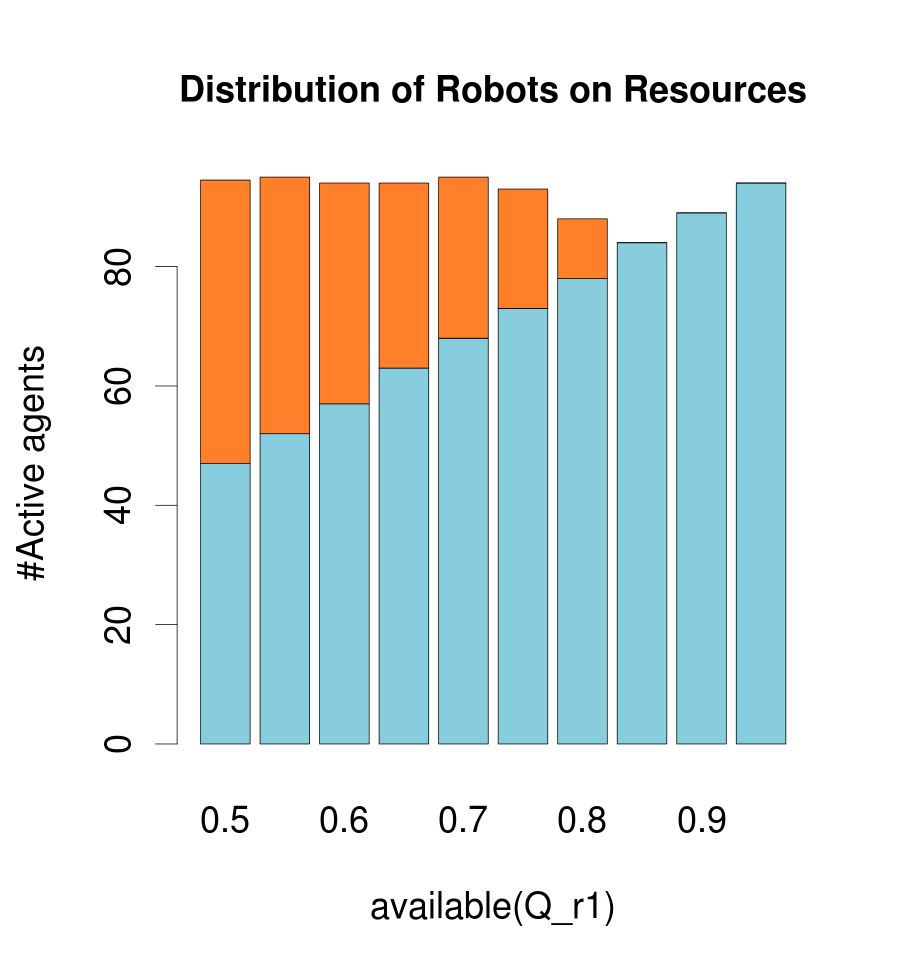
\includegraphics[width=\imgSize]{../images/5StaticEnv/barplotAliveR1AndR2_median_env1}i\\
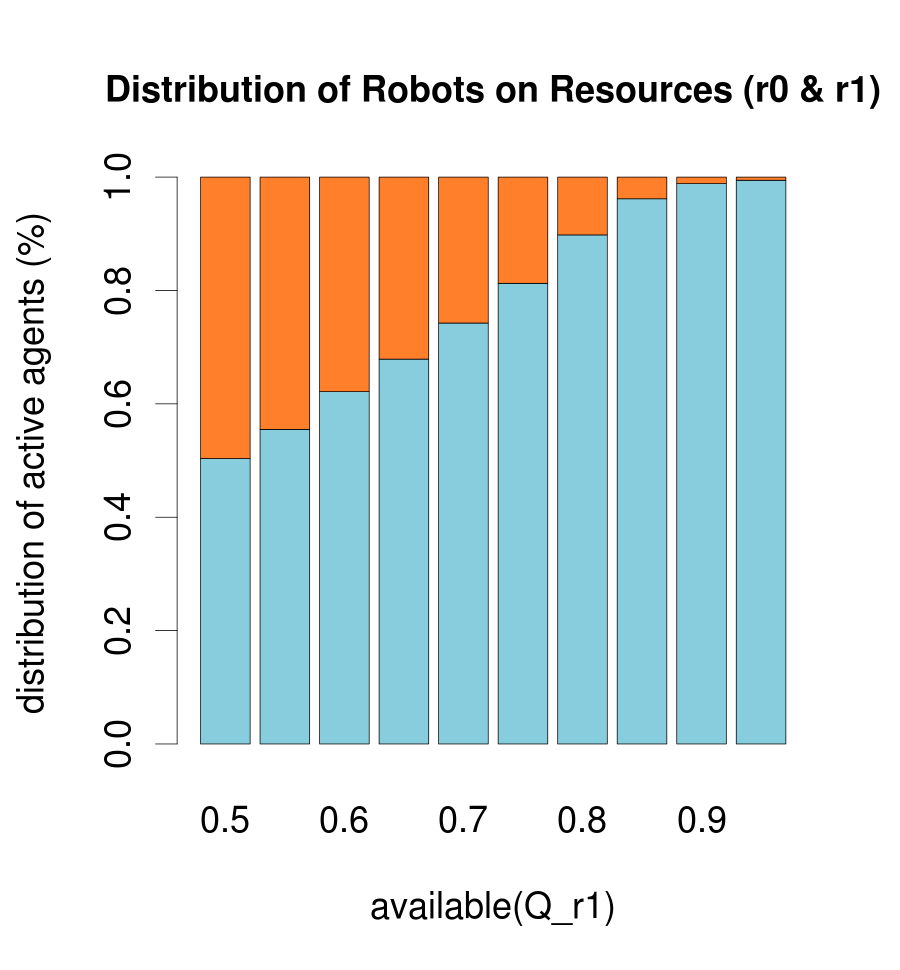
\includegraphics[width=\imgSize]{../images/5StaticEnv/barplotAliveR1AndR2_mean_env1_normalized}& 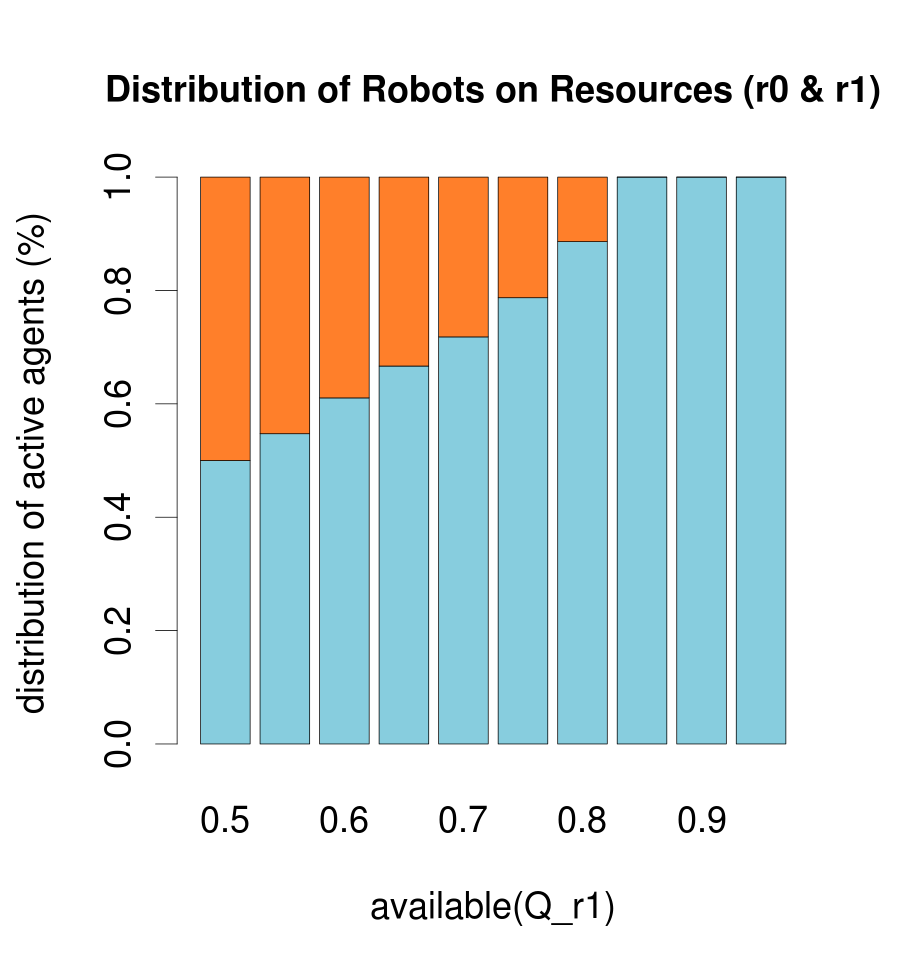
\includegraphics[width=\imgSize]{../images/5StaticEnv/barplotAliveR1AndR2_median_env1_normalized}
\end{tabular}
\end{table}

\begin{table}[H]
\caption{Environment 1, Samples}
\centering
\begin{tabular}{cc}
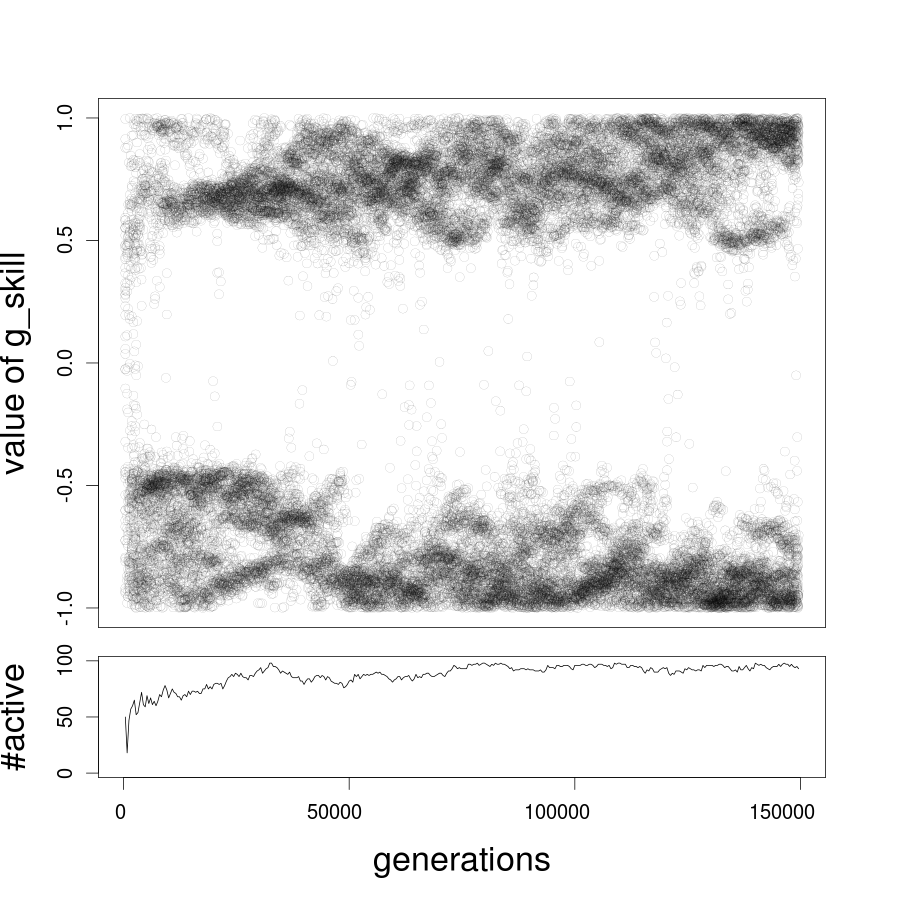
\includegraphics[width=\imgSize]{../images/5StaticEnv/Gplot47_staticEnv1}&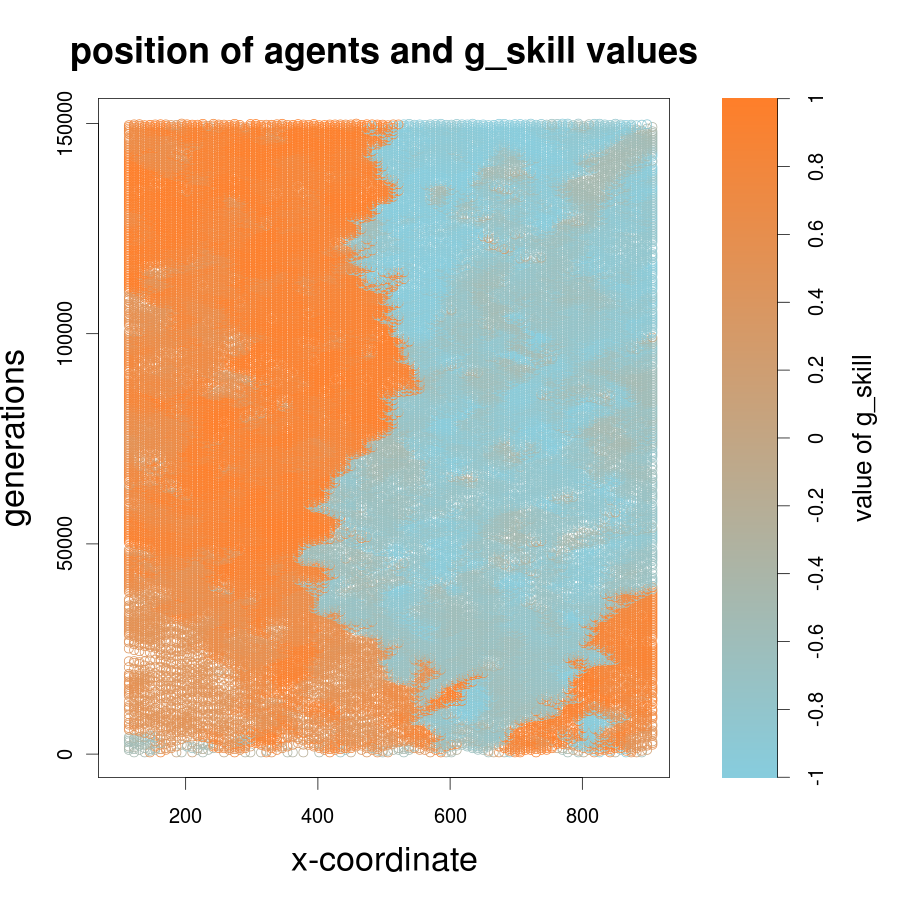
\includegraphics[width=\imgSize]{../images/5StaticEnv/Gplot47Static_staticEnv1}\\
\newline
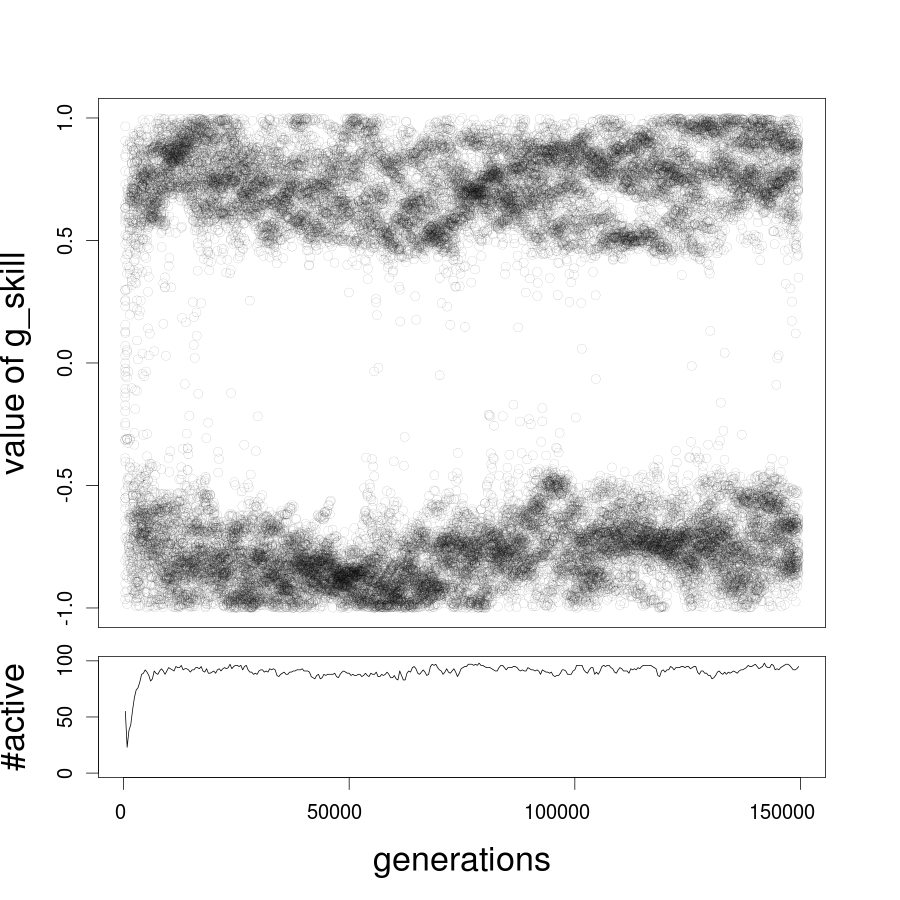
\includegraphics[width=\imgSize]{../images/5StaticEnv/Gplot66_staticEnv1}&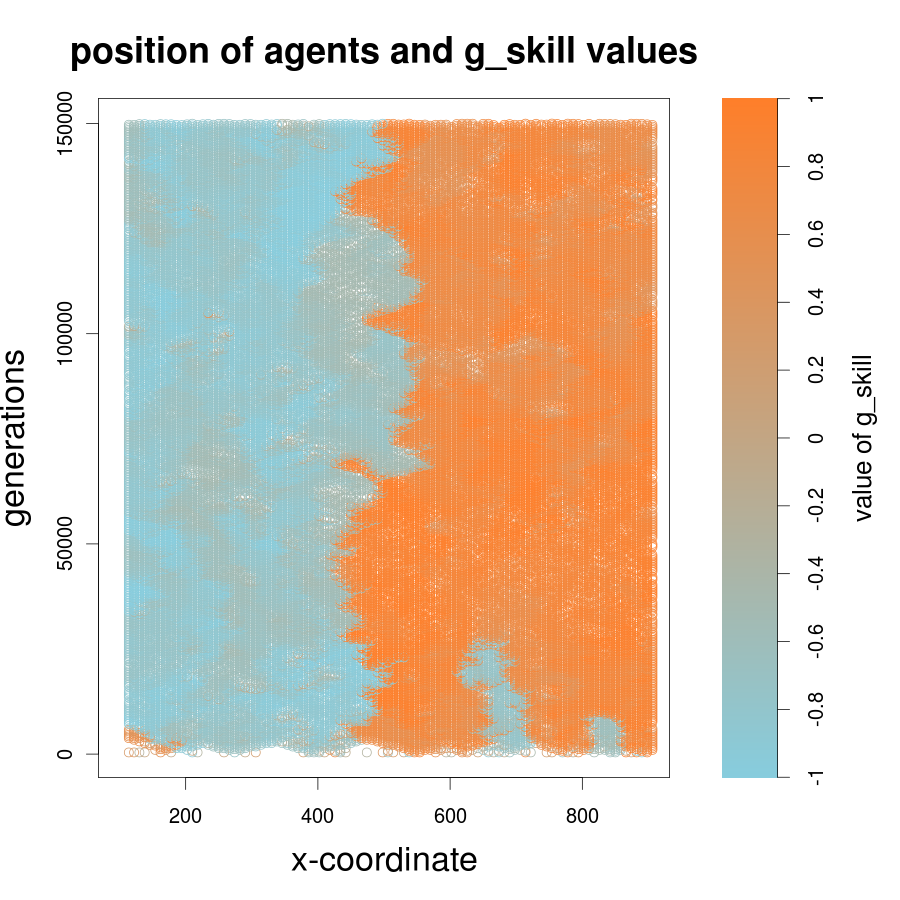
\includegraphics[width=\imgSize]{../images/5StaticEnv/Gplot66Static_staticEnv1}\\
\end{tabular}
\end{table}
\begin{table}[H]
\begin{tabular}{cc}
 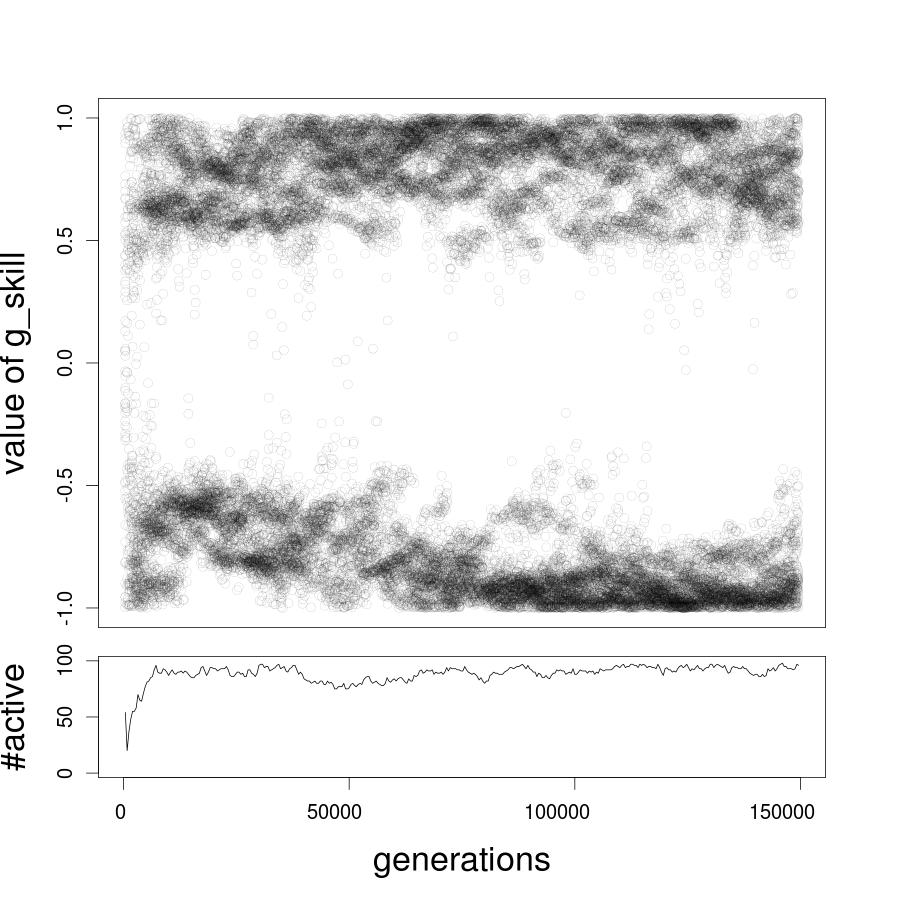
\includegraphics[width=\imgSize]{../images/5StaticEnv/Gplot29_staticEnv1}&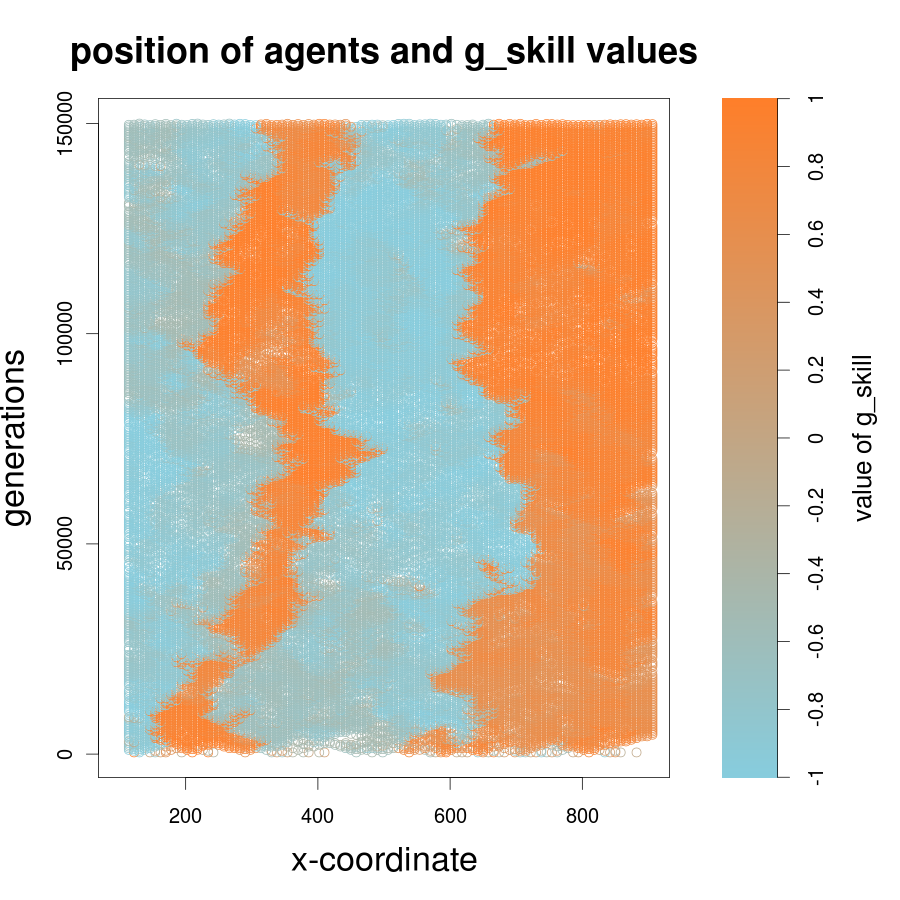
\includegraphics[width=\imgSize]{../images/5StaticEnv/Gplot29Static_staticEnv1}\\
 \newline
 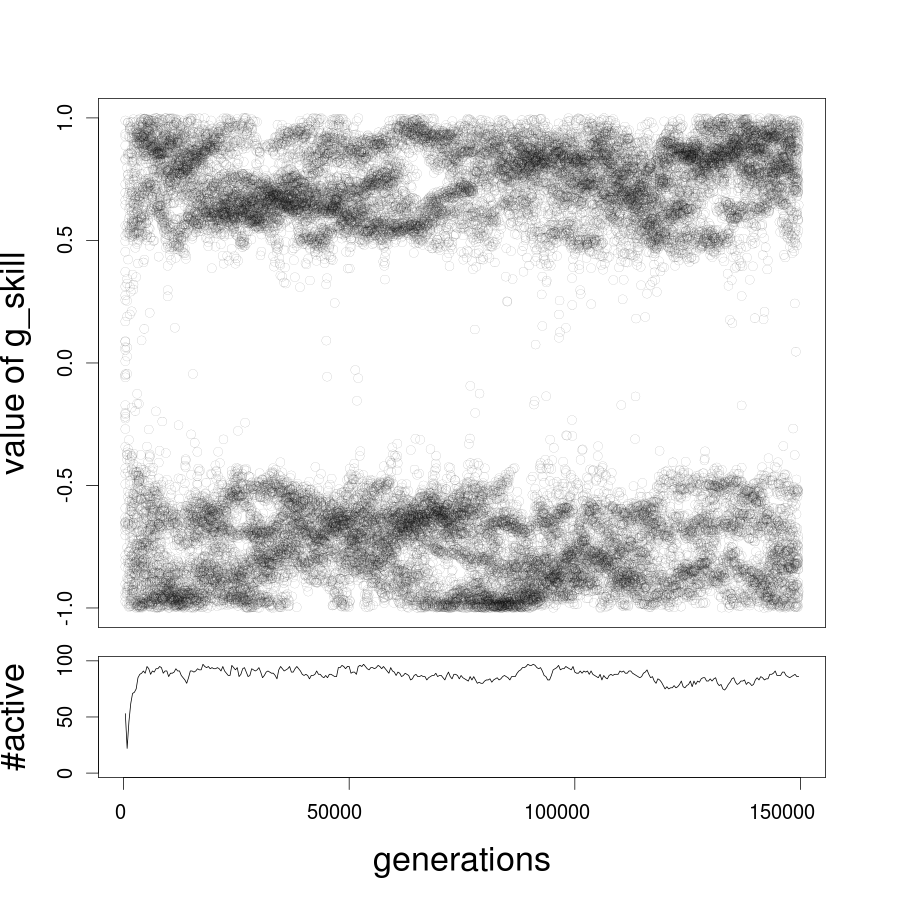
\includegraphics[width=\imgSize]{../images/5StaticEnv/Gplot9_staticEnv1}&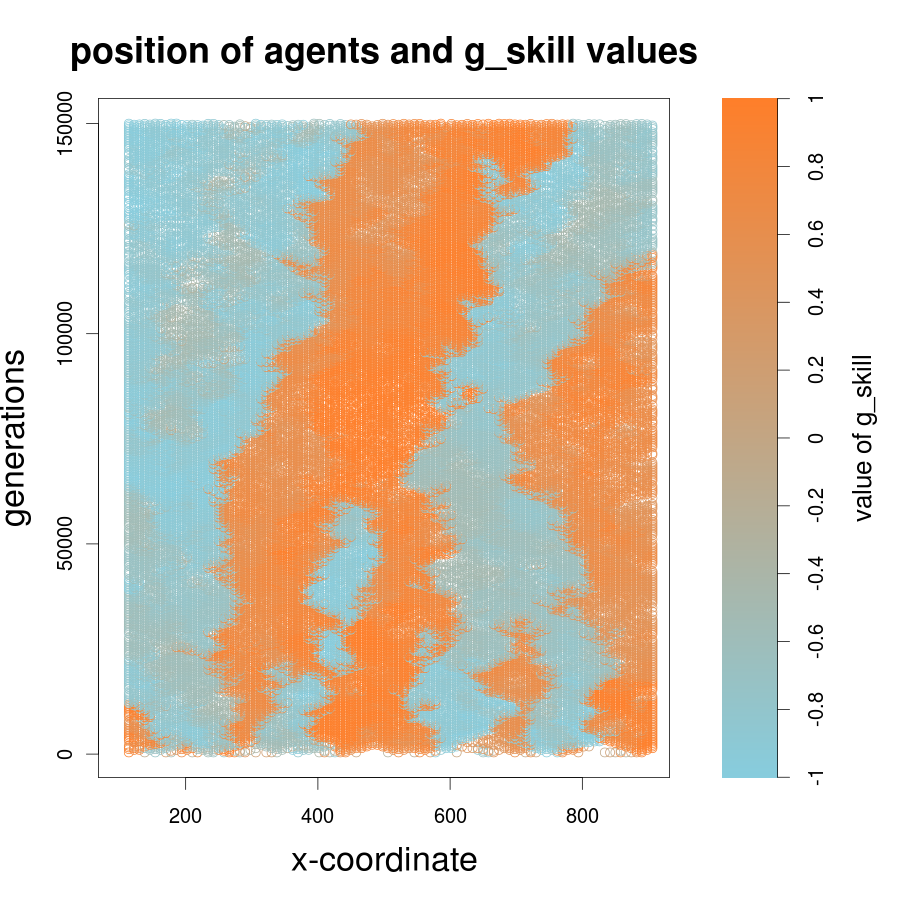
\includegraphics[width=\imgSize]{../images/5StaticEnv/Gplot9Static_staticEnv1}\\
\end{tabular}

\end{table}


\subsubsection{Static environment 2}
\begin{table}[H]
\caption{results for ENV2}
\centering
\begin{tabular}{cc}
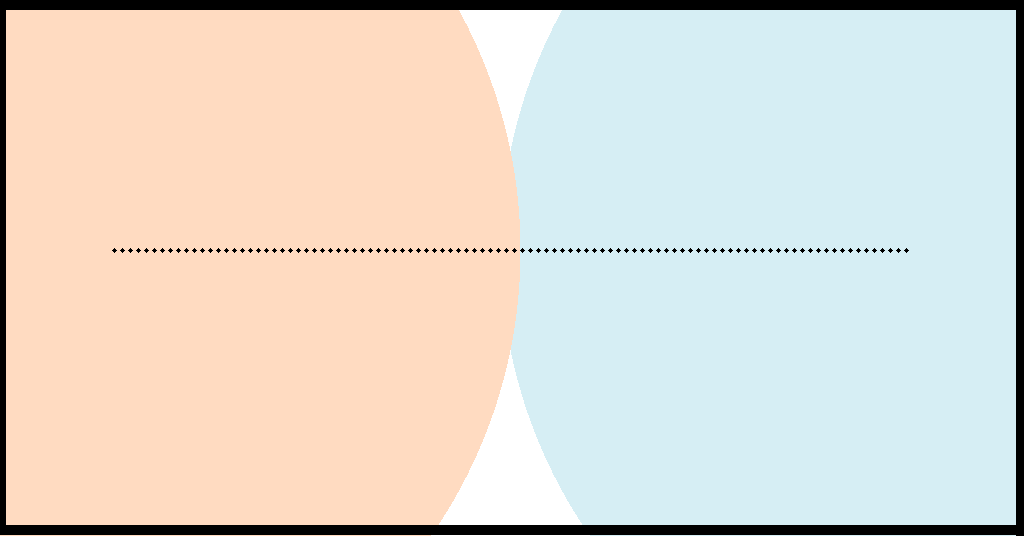
\includegraphics[width=\imgSize]{../images/5StaticEnv/environments/staticEnv2}&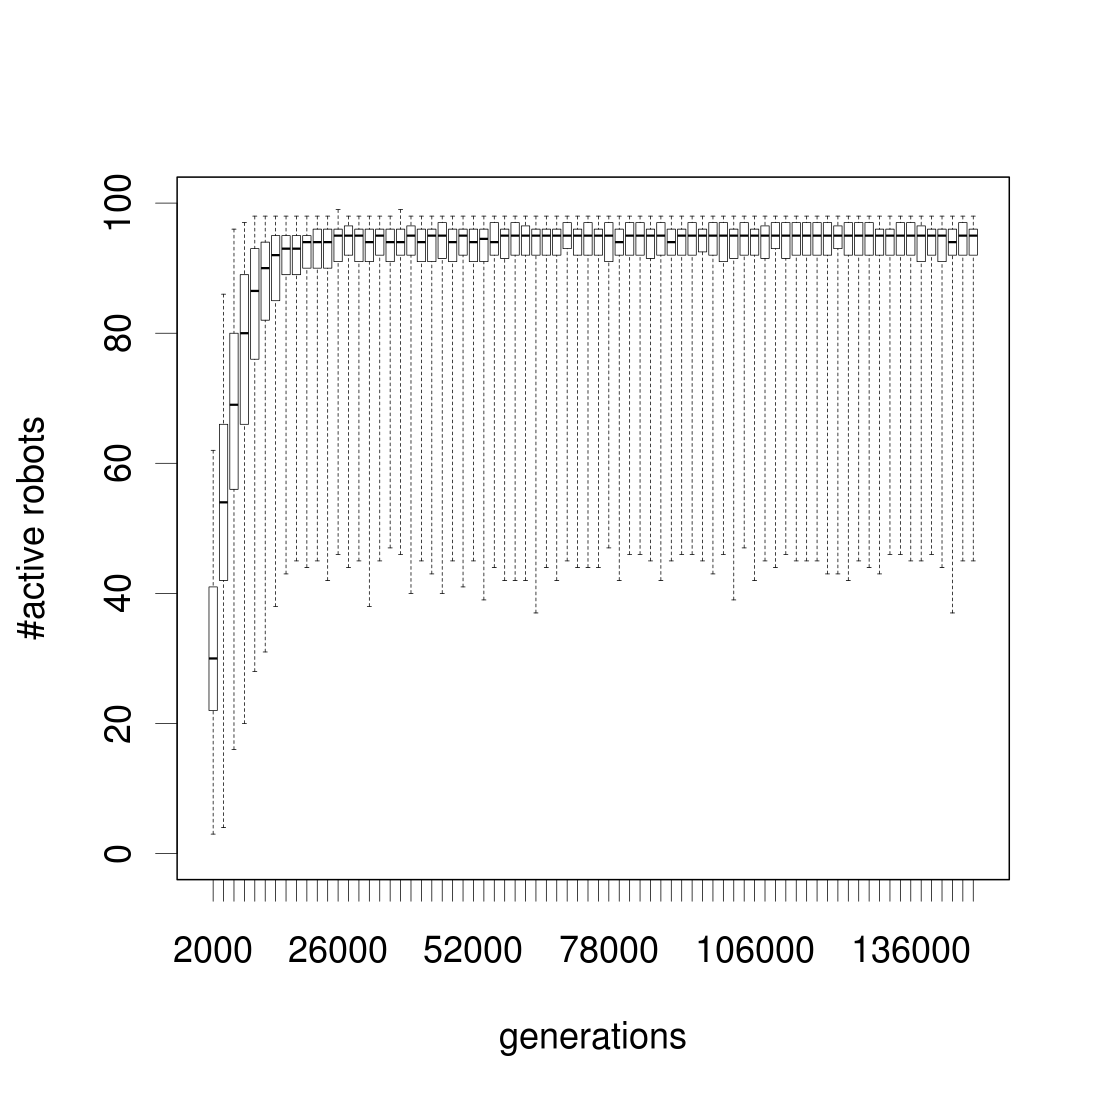
\includegraphics[width=\imgSize]{../images/5StaticEnv/alive_staticEnv2}\\
\newline
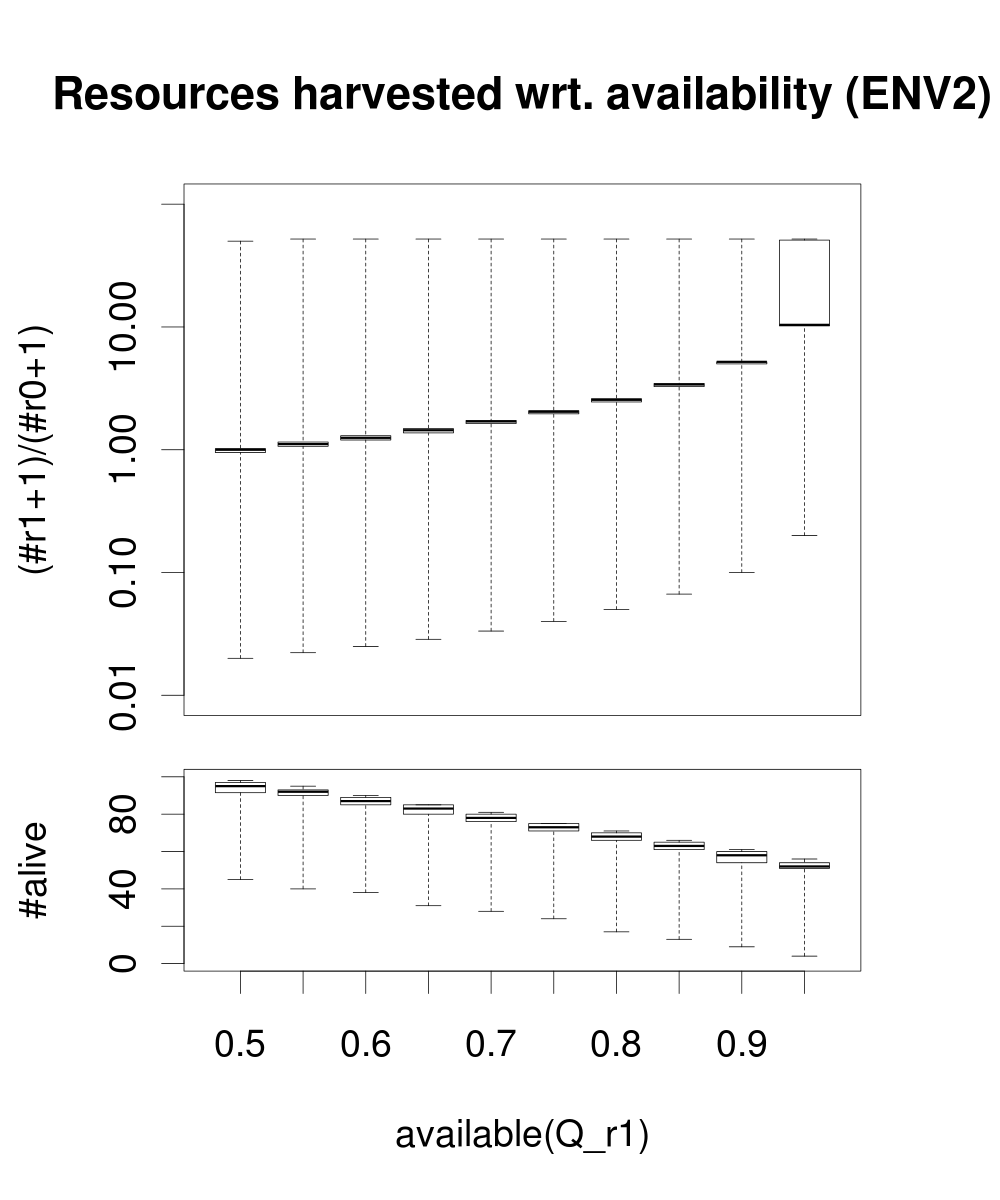
\includegraphics[width=\imgSize]{../images/5StaticEnv/ratioAndRep_staticEnv2LogY}&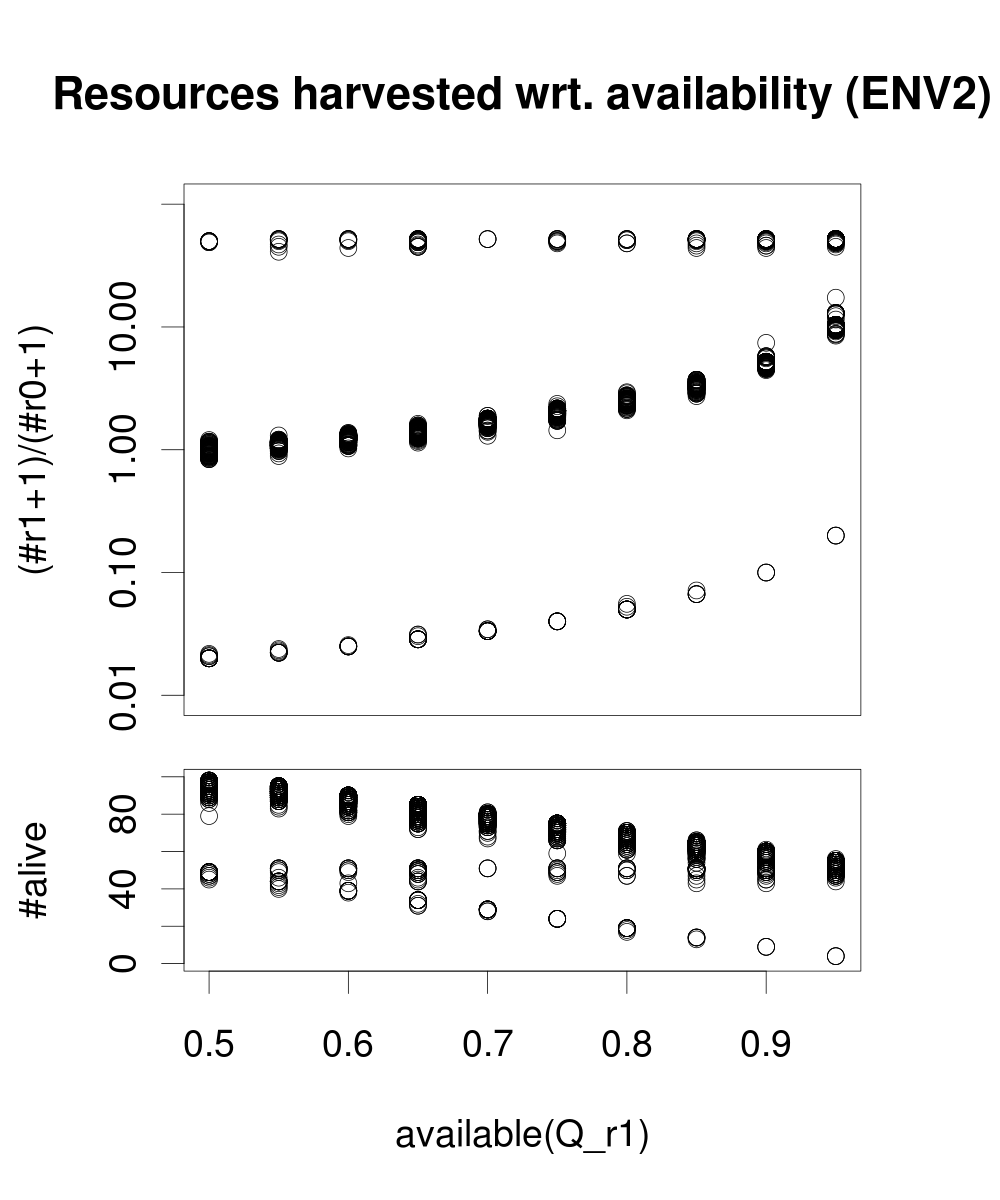
\includegraphics[width=\imgSize]{../images/5StaticEnv/ratioAndRep_staticEnvPlot2LogY}\\
\end{tabular}
\end{table}
\begin{table}[H]
\caption{Left graphs use mean values ; rights use the median.Bottom graphes are normalized}
\begin{tabular}{cc}

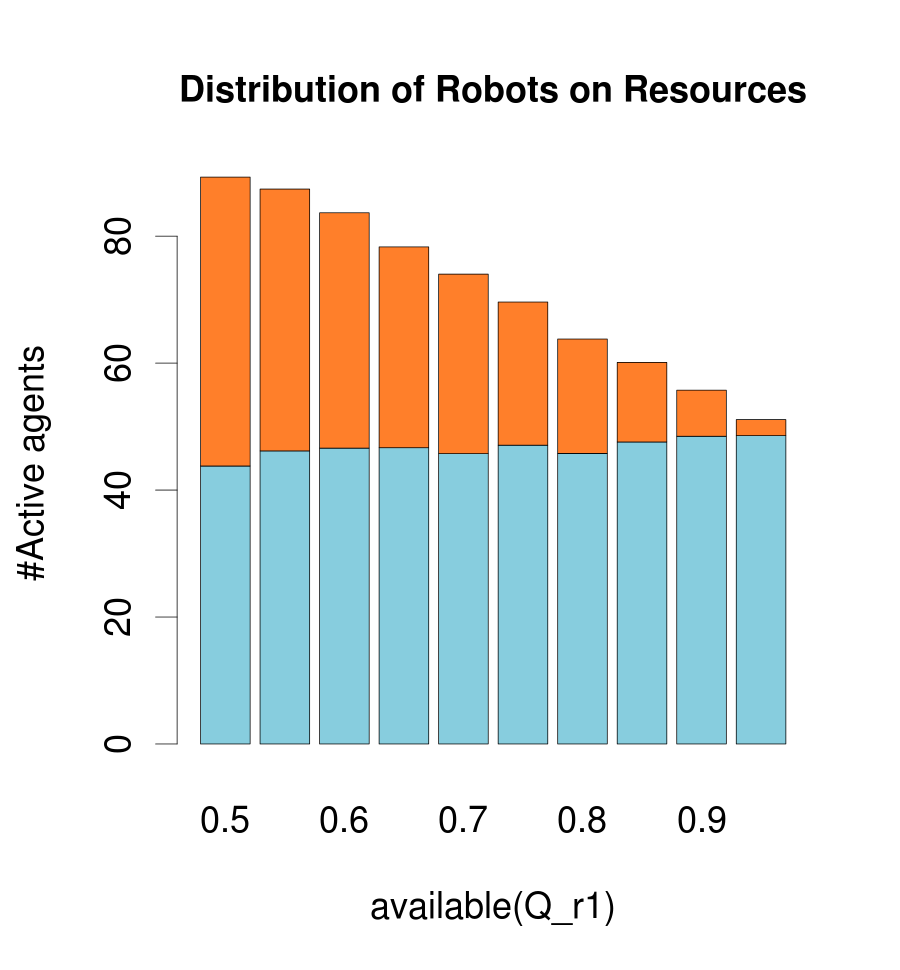
\includegraphics[width=\imgSize]{../images/5StaticEnv/barplotAliveR1AndR2_mean_env2}& 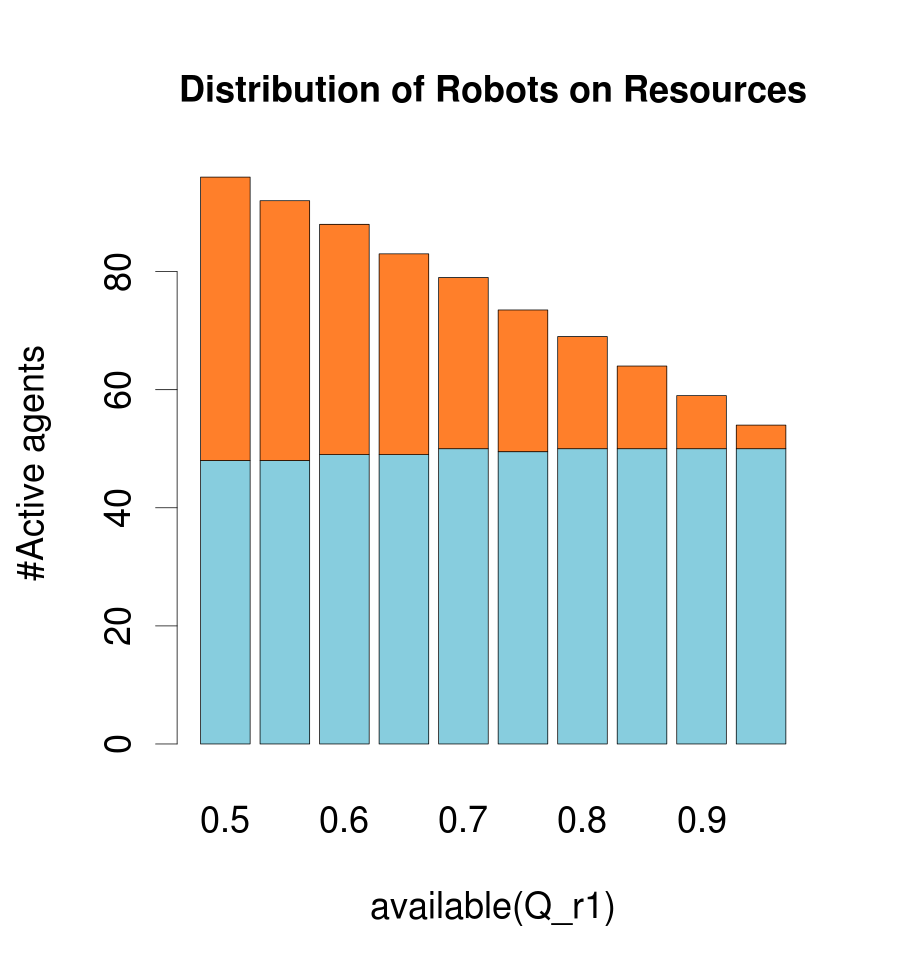
\includegraphics[width=\imgSize]{../images/5StaticEnv/barplotAliveR1AndR2_median_env2}\\
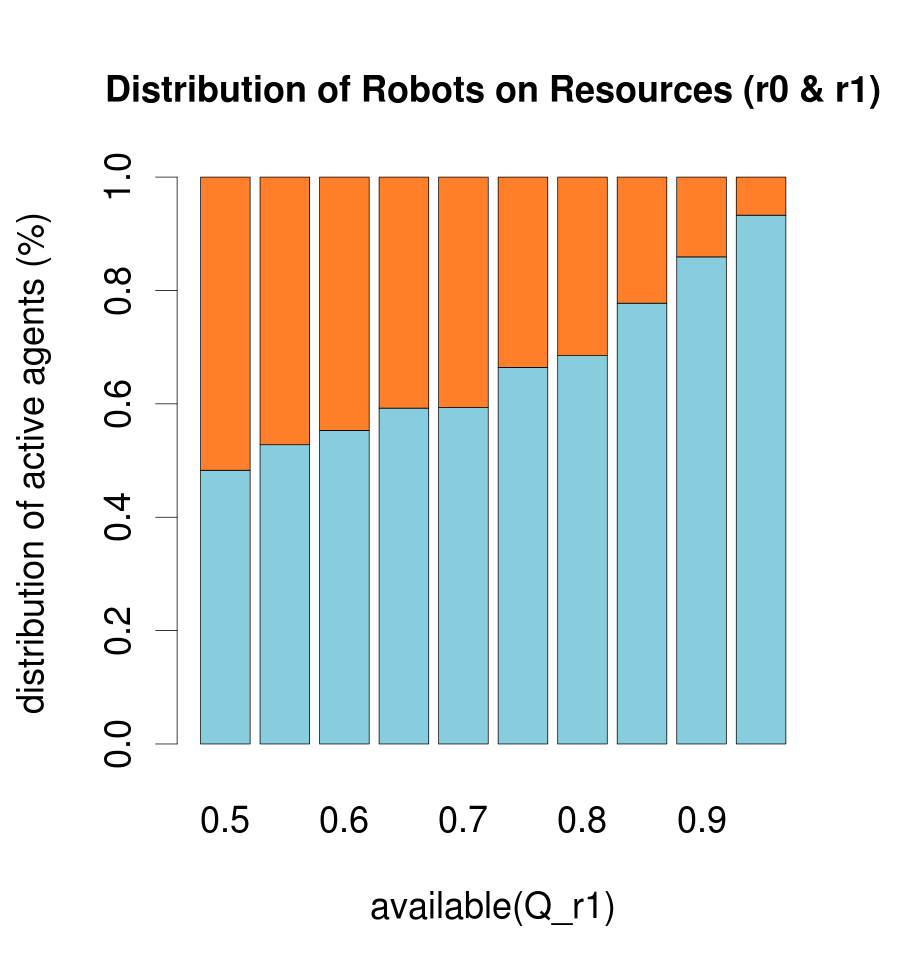
\includegraphics[width=\imgSize]{../images/5StaticEnv/barplotAliveR1AndR2_mean_env2_normalized}& 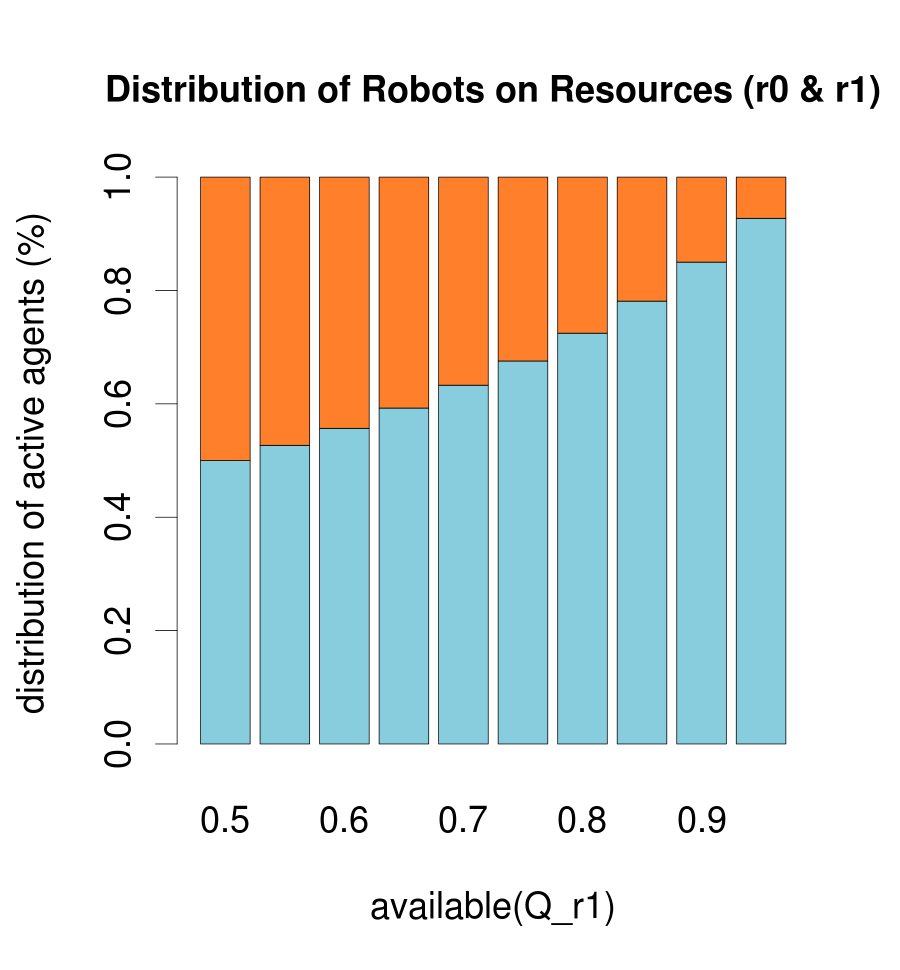
\includegraphics[width=\imgSize]{../images/5StaticEnv/barplotAliveR1AndR2_median_env2_normalized}
\end{tabular} 
\end{table}
 \begin{table}[H]
 \caption{Environment 2, Samples: \\The environmental setup (the reward function) does not allow a group to switch in a other one ; maybe the fitness gap beetwen the two phenotype is to wide.  } \centering 
\begin{tabular}{cc} 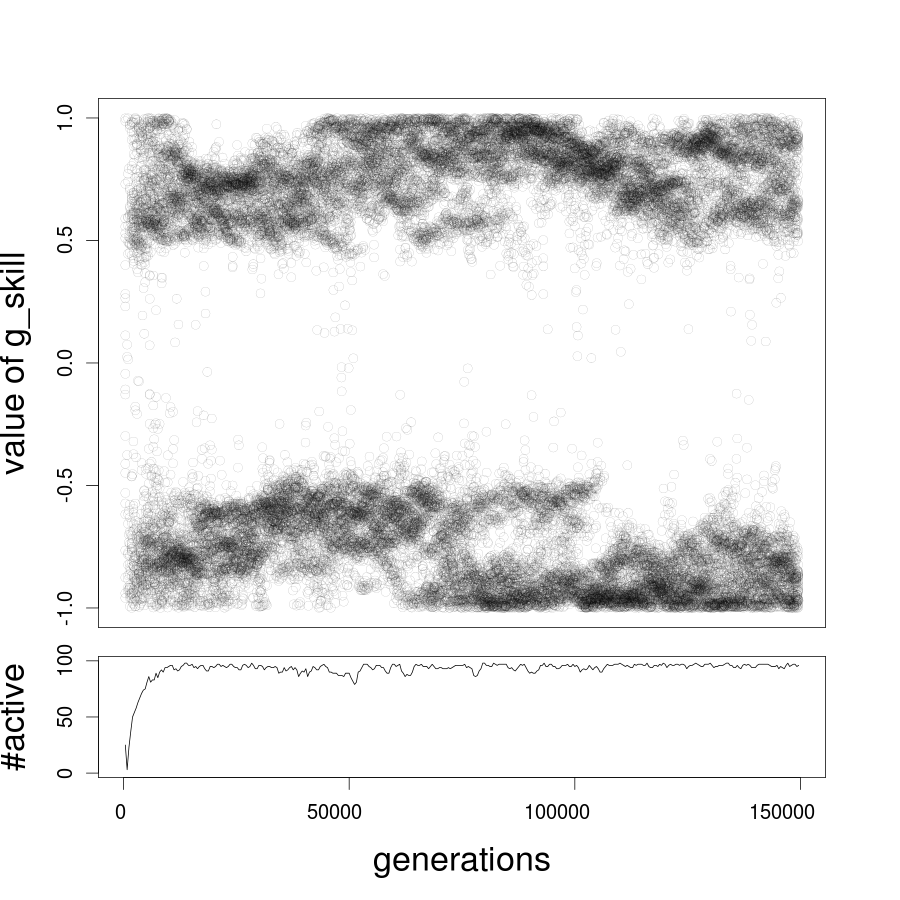
\includegraphics[width=\imgSize]{../images/5StaticEnv/Gplot22_staticEnv2}&\includegraphics[width=\imgSize]{../images/5StaticEnv/Gplot22Static_staticEnv2}\\ \newline \includegraphics[width=\imgSize]{../images/5StaticEnv/Gplot66_staticEnv2}&\includegraphics[width=\imgSize]{../images/5StaticEnv/Gplot66Static_staticEnv2}\\ \end{tabular} \end{table} \begin{table}[H] \begin{tabular}{cc} \includegraphics[width=\imgSize]{../images/5StaticEnv/Gplot5_staticEnv2}&\includegraphics[width=\imgSize]{../images/5StaticEnv/Gplot5Static_staticEnv2}\\ \newline \includegraphics[width=\imgSize]{../images/5StaticEnv/Gplot92_staticEnv2}&\includegraphics[width=\imgSize]{../images/5StaticEnv/Gplot92Static_staticEnv2}\\ \end{tabular} \end{table} \subsubsection{Static environment 3} \begin{table}[H] \caption{results for env3} \centering \begin{tabular}{cc} \includegraphics[width=\imgSize]{../images/5StaticEnv/environments/staticEnv3}&\includegraphics[width=\imgSize]{../images/5StaticEnv/alive_staticEnv3}\\ \newline \includegraphics[width=\imgSize]{../images/5StaticEnv/ratioAndRep_staticEnv3LogY}&\includegraphics[width=\imgSize]{../images/5StaticEnv/ratioAndRep_staticEnvPlot3LogY}\\ \end{tabular} \end{table}
\begin{table}[H]
\caption{Left graphs use mean values ; rights use the median.Bottom graphes are normalized}
\begin{tabular}{cc}
\includegraphics[width=\imgSize]{../images/5StaticEnv/barplotAliveR1AndR2_mean_env3}& \includegraphics[width=\imgSize]{../images/5StaticEnv/barplotAliveR1AndR2_median_env3}\\
\includegraphics[width=\imgSize]{../images/5StaticEnv/barplotAliveR1AndR2_mean_env3_normalized}& \includegraphics[width=\imgSize]{../images/5StaticEnv/barplotAliveR1AndR2_median_env3_normalized}
\end{tabular}

\end{table}

\begin{table}[H]
\caption{Environment 3, Samples}
\centering
\begin{tabular}{cc}
\includegraphics[width=\imgSize]{../images/5StaticEnv/Gplot5_staticEnv3}&\includegraphics[width=\imgSize]{../images/5StaticEnv/Gplot5Static_staticEnv3}\\
\newline
\includegraphics[width=\imgSize]{../images/5StaticEnv/Gplot8_staticEnv3}&\includegraphics[width=\imgSize]{../images/5StaticEnv/Gplot8Static_staticEnv3}\\
\end{tabular}
\end{table}
\begin{table}[H]
\begin{tabular}{cc}
 \includegraphics[width=\imgSize]{../images/5StaticEnv/Gplot51_staticEnv3}&\includegraphics[width=\imgSize]{../images/5StaticEnv/Gplot51Static_staticEnv3}\\
 \newline
 \includegraphics[width=\imgSize]{../images/5StaticEnv/Gplot99_staticEnv3}&\includegraphics[width=\imgSize]{../images/5StaticEnv/Gplot99Static_staticEnv3}\\
\end{tabular}

\end{table}

\subsubsection{Static environment 4}

\begin{table}[H]
\caption{results for env4}
\centering
\begin{tabular}{cc}
\includegraphics[width=\imgSize]{../images/5StaticEnv/environments/staticEnv4}&\includegraphics[width=\imgSize]{../images/5StaticEnv/alive_staticEnv4}\\
\newline
\includegraphics[width=\imgSize]{../images/5StaticEnv/ratioAndRep_staticEnv4LogY}&\includegraphics[width=\imgSize]{../images/5StaticEnv/ratioAndRep_staticEnvPlot4LogY}\\
\end{tabular}
\end{table}
\begin{table}[H]
\caption{Left graphs use mean values ; rights use the median.Bottom graphes are normalized}
\begin{tabular}{cc}
\includegraphics[width=\imgSize]{../images/5StaticEnv/barplotAliveR1AndR2_mean_env4}& \includegraphics[width=\imgSize]{../images/5StaticEnv/barplotAliveR1AndR2_median_env4}\\
\includegraphics[width=\imgSize]{../images/5StaticEnv/barplotAliveR1AndR2_mean_env4_normalized}& \includegraphics[width=\imgSize]{../images/5StaticEnv/barplotAliveR1AndR2_median_env4_normalized}
\end{tabular}
\end{table}
\begin{table}[H]
\caption{Environment 4, Samples}
\centering
\begin{tabular}{cc}
\includegraphics[width=\imgSize]{../images/5StaticEnv/Gplot17_staticEnv4}&\includegraphics[width=\imgSize]{../images/5StaticEnv/Gplot17Static_staticEnv4}\\
\newline
\includegraphics[width=\imgSize]{../images/5StaticEnv/Gplot40_staticEnv4}&\includegraphics[width=\imgSize]{../images/5StaticEnv/Gplot40Static_staticEnv4}\\
\end{tabular}
\end{table}
\begin{table}[H]
\begin{tabular}{cc}
 \includegraphics[width=\imgSize]{../images/5StaticEnv/Gplot62_staticEnv4}&\includegraphics[width=\imgSize]{../images/5StaticEnv/Gplot62Static_staticEnv4}\\
 \newline
 \includegraphics[width=\imgSize]{../images/5StaticEnv/Gplot58_staticEnv4}&\includegraphics[width=\imgSize]{../images/5StaticEnv/Gplot58Static_staticEnv4}\\
\end{tabular}

\end{table}

\begin{table}[H]
\centering
\caption{À gauche les moyennes des rapports (les écarts types sont trops importants, sachant que parfois le rapport est assez faible : il y a deux sous populations ; parfois il est proche de 100 : il n'y a qu'une population, ce qui brouille beaucoup le graphe), à droite les rapports théoriques si les deux populations étaient réparties parfaitement pour utiliser l'environnement au mieux. On voit que là où les deux resources sont accessible simultanéments (env0, 1 et 3), plus les individus sont connectés (env0 et env3) plus il est difficile de maintenir un ratio proche du ratio théorique.}
\begin{tabular}{cc}
\includegraphics[height=\imgSize]{../images/5StaticEnv/ratioR1R2foreachEnv}&\includegraphics[height=\imgSize]{../images/5StaticEnv/theroticalRatios.png}\\
\newline
\end{tabular}
\end{table}

\subsection{For all sparsity in random pseudo-networks}


\begin{table}[H]
\caption{Speciation capacities depending on the sparsities of the communcation network}
% \caption{pourcentage }
\centering
\begin{tabular}{lcc}
resource & median & mean\\
R1 & \includegraphics[width=\imgSize]{images/R1_median}&\includegraphics[width=\imgSize]{images/R1_mean}\\
R0 & \includegraphics[width=\imgSize]{images/R0_median}&\includegraphics[width=\imgSize]{images/R0_mean}\\
total & \includegraphics[width=\imgSize]{images/active_median}&\includegraphics[width=\imgSize]{images/active_mean}
\end{tabular}

\end{table}

When can have a look on some noticeable parts of the 3d plot. 

\begin{itemize}
\item slice through the $Q_{r1}$'s availablities axis : 
\begin{figure}[H]
\caption{\#Active wrt. density }
\caption{harvest($Q_{r1}$ wrt. density }
\subfloat[availability($Q_{r1}$)=.50]{\includegraphics[width=\imgSize]{images/alive_density_r1-50.png}}
\subfloat[availability($Q_{r1}$)=.70]{\includegraphics[width=\imgSize]{images/alive_density_r1-70.png}}\\
\subfloat[availability($Q_{r1}$)=.90]{\includegraphics[width=\imgSize]{images/alive_density_r1-90.png}}
\subfloat[]{\includegraphics[width=\imgSize]{images/active_median}}
\end{figure}
\begin{figure}[H]
\caption{harvest($Q_{r1}$ wrt. density }
\subfloat[availability($Q_{r1}$)=.50]{\includegraphics[width=\imgSize]{images/harvestr1_density_r1-50.png}}
\subfloat[availability($Q_{r1}$)=.70]{\includegraphics[width=\imgSize]{images/harvestr1_density_r1-70.png}}\\
\subfloat[availability($Q_{r1}$)=.90]{\includegraphics[width=\imgSize]{images/harvestr1_density_r1-90.png}}
\subfloat[]{\includegraphics[width=\imgSize]{images/R1_median}}
\end{figure}

\item slice through the density axis : 
\begin{figure}[H]
\caption{\#active agents wrt. available($Q_{r1}$)}
\subfloat[density=0.02]{\includegraphics[width=\imgSize]{images/alive_r1_density-2.png}}
\subfloat[density=0.08]{\includegraphics[width=\imgSize]{images/alive_r1_density-8.png}}\\
\subfloat[density=0.60]{\includegraphics[width=\imgSize]{images/alive_r1_density-60.png}}
\subfloat[]{\includegraphics[width=\imgSize]{images/active_median}}

\end{figure}
\begin{figure}[H]
\caption{harvest($Q_{r1}$) wrt. available($Q_{r1}$):}
\subfloat[density=0.02]{\includegraphics[width=\imgSize]{images/harvestr1_r1_density-2.png}}
\subfloat[density=0.08]{\includegraphics[width=\imgSize]{images/harvestr1_r1_density-8.png}}\\
\subfloat[density=0.60]{\includegraphics[width=\imgSize]{images/harvestr1_r1_density-60.png}}
\subfloat[]{\includegraphics[width=\imgSize]{images/R1_median}}

\end{figure}
\end{itemize}

\section{Discussion}

\bibliographystyle{apalike}
\addcontentsline{toc}{chapter}{Bibliographie}
\bibliography{../../../../Doc/bib/simon.bib,../../../../Doc/bib/nicolas.bib,../../../../Doc/bib/jeanmarc.bib}


\end{document}
